% Options for packages loaded elsewhere
\PassOptionsToPackage{unicode}{hyperref}
\PassOptionsToPackage{hyphens}{url}
\PassOptionsToPackage{dvipsnames,svgnames*,x11names*}{xcolor}
%
\documentclass[
  10pt,
  dvipsnames,enabledeprecatedfontcommands]{scrartcl}
\usepackage{amsmath,amssymb}
\usepackage{lmodern}
\usepackage{ifxetex,ifluatex}
\ifnum 0\ifxetex 1\fi\ifluatex 1\fi=0 % if pdftex
  \usepackage[T1]{fontenc}
  \usepackage[utf8]{inputenc}
  \usepackage{textcomp} % provide euro and other symbols
\else % if luatex or xetex
  \usepackage{unicode-math}
  \defaultfontfeatures{Scale=MatchLowercase}
  \defaultfontfeatures[\rmfamily]{Ligatures=TeX,Scale=1}
\fi
% Use upquote if available, for straight quotes in verbatim environments
\IfFileExists{upquote.sty}{\usepackage{upquote}}{}
\IfFileExists{microtype.sty}{% use microtype if available
  \usepackage[]{microtype}
  \UseMicrotypeSet[protrusion]{basicmath} % disable protrusion for tt fonts
}{}
\usepackage{xcolor}
\IfFileExists{xurl.sty}{\usepackage{xurl}}{} % add URL line breaks if available
\IfFileExists{bookmark.sty}{\usepackage{bookmark}}{\usepackage{hyperref}}
\hypersetup{
  pdftitle={Likelihood ratio and evidence strength},
  pdfauthor={Marcello Di Bello and Rafal Urbaniak},
  colorlinks=true,
  linkcolor=Maroon,
  filecolor=Maroon,
  citecolor=Blue,
  urlcolor=blue,
  pdfcreator={LaTeX via pandoc}}
\urlstyle{same} % disable monospaced font for URLs
\usepackage{graphicx}
\makeatletter
\def\maxwidth{\ifdim\Gin@nat@width>\linewidth\linewidth\else\Gin@nat@width\fi}
\def\maxheight{\ifdim\Gin@nat@height>\textheight\textheight\else\Gin@nat@height\fi}
\makeatother
% Scale images if necessary, so that they will not overflow the page
% margins by default, and it is still possible to overwrite the defaults
% using explicit options in \includegraphics[width, height, ...]{}
\setkeys{Gin}{width=\maxwidth,height=\maxheight,keepaspectratio}
% Set default figure placement to htbp
\makeatletter
\def\fps@figure{htbp}
\makeatother
\setlength{\emergencystretch}{3em} % prevent overfull lines
\providecommand{\tightlist}{%
  \setlength{\itemsep}{0pt}\setlength{\parskip}{0pt}}
\setcounter{secnumdepth}{5}
%\documentclass{article}

% %packages
 \usepackage{booktabs}
\usepackage{subcaption}
\usepackage{multirow}
\usepackage{colortbl}
\usepackage{graphicx}
\usepackage{longtable}
\usepackage{ragged2e}
\usepackage{etex}
%\usepackage{yfonts}
\usepackage{marvosym}
\usepackage[notextcomp]{kpfonts}
\usepackage{nicefrac}
\newcommand*{\QED}{\hfill \footnotesize {\sc Q.e.d.}}
\usepackage{floatrow}
%\usepackage[titletoc]{appendix}
%\renewcommand\thesubsection{\Alph{subsection}}

\usepackage[textsize=footnotesize]{todonotes}
\newcommand{\ali}[1]{\todo[color=gray!40]{#1}}
\newcommand{\mar}[1]{\todo[color=blue!40]{#1}}
\newcommand{\raf}[1]{\todo[color=olive!40]{#1}}
%\linespread{1.5}
\newcommand{\indep}{\!\perp \!\!\! \perp\!}


\setlength{\parindent}{10pt}
\setlength{\parskip}{1pt}


%language
\usepackage{times}
\usepackage{t1enc}
%\usepackage[utf8x]{inputenc}
%\usepackage[polish]{babel}
%\usepackage{polski}




%AMS
\usepackage{amsfonts}
\usepackage{amssymb}
\usepackage{amsthm}
\usepackage{amsmath}
\usepackage{mathtools}

\usepackage{geometry}
 \geometry{a4paper,left=35mm,top=20mm,}


%environments
\newtheorem{fact}{Fact}



%abbreviations
\newcommand{\ra}{\rangle}
\newcommand{\la}{\langle}
\newcommand{\n}{\neg}
\newcommand{\et}{\wedge}
\newcommand{\jt}{\rightarrow}
\newcommand{\ko}[1]{\forall  #1\,}
\newcommand{\ro}{\leftrightarrow}
\newcommand{\exi}[1]{\exists\, {_{#1}}}
\newcommand{\pr}[1]{\mathsf{P}(#1)}
\newcommand{\cost}{\mathsf{cost}}
\newcommand{\benefit}{\mathsf{benefit}}
\newcommand{\ut}{\mathsf{ut}}

\newcommand{\odds}{\mathsf{Odds}}
\newcommand{\ind}{\mathsf{Ind}}
\newcommand{\nf}[2]{\nicefrac{#1\,}{#2}}
\newcommand{\R}[1]{\texttt{#1}}
\newcommand{\prr}[1]{\mbox{$\mathtt{P}_{prior}(#1)$}}
\newcommand{\prp}[1]{\mbox{$\mathtt{P}_{posterior}(#1)$}}



\newtheorem{q}{\color{blue}Question}
\newtheorem{lemma}{Lemma}
\newtheorem{theorem}{Theorem}



%technical intermezzo
%---------------------

\newcommand{\intermezzoa}{
	\begin{minipage}[c]{13cm}
	\begin{center}\rule{10cm}{0.4pt}



	\tiny{\sc Optional Content Starts}
	
	\vspace{-1mm}
	
	\rule{10cm}{0.4pt}\end{center}
	\end{minipage}\nopagebreak 
	}


\newcommand{\intermezzob}{\nopagebreak 
	\begin{minipage}[c]{13cm}
	\begin{center}\rule{10cm}{0.4pt}

	\tiny{\sc Optional Content Ends}
	
	\vspace{-1mm}
	
	\rule{10cm}{0.4pt}\end{center}
	\end{minipage}
	}
%--------------------






















\newtheorem*{reply*}{Reply}
\usepackage{enumitem}
\newcommand{\question}[1]{\begin{enumerate}[resume,leftmargin=0cm,labelsep=0cm,align=left]
\item #1
\end{enumerate}}

\usepackage{float}

% \setbeamertemplate{blocks}[rounded][shadow=true]
% \setbeamertemplate{itemize items}[ball]
% \AtBeginPart{}
% \AtBeginSection{}
% \AtBeginSubsection{}
% \AtBeginSubsubsection{}
% \setlength{\emergencystretch}{0em}
% \setlength{\parskip}{0pt}






\usepackage[authoryear]{natbib}

%\bibliographystyle{apalike}



\usepackage{tikz}
\usetikzlibrary{positioning,shapes,arrows}

\usepackage{booktabs}
\usepackage{longtable}
\usepackage{array}
\usepackage{multirow}
\usepackage{wrapfig}
\usepackage{float}
\usepackage{colortbl}
\usepackage{pdflscape}
\usepackage{tabu}
\usepackage{threeparttable}
\usepackage{threeparttablex}
\usepackage[normalem]{ulem}
\usepackage{makecell}
\usepackage{xcolor}
\ifluatex
  \usepackage{selnolig}  % disable illegal ligatures
\fi
\newlength{\cslhangindent}
\setlength{\cslhangindent}{1.5em}
\newlength{\csllabelwidth}
\setlength{\csllabelwidth}{3em}
\newenvironment{CSLReferences}[2] % #1 hanging-ident, #2 entry spacing
 {% don't indent paragraphs
  \setlength{\parindent}{0pt}
  % turn on hanging indent if param 1 is 1
  \ifodd #1 \everypar{\setlength{\hangindent}{\cslhangindent}}\ignorespaces\fi
  % set entry spacing
  \ifnum #2 > 0
  \setlength{\parskip}{#2\baselineskip}
  \fi
 }%
 {}
\usepackage{calc}
\newcommand{\CSLBlock}[1]{#1\hfill\break}
\newcommand{\CSLLeftMargin}[1]{\parbox[t]{\csllabelwidth}{#1}}
\newcommand{\CSLRightInline}[1]{\parbox[t]{\linewidth - \csllabelwidth}{#1}\break}
\newcommand{\CSLIndent}[1]{\hspace{\cslhangindent}#1}

\title{Likelihood ratio and evidence strength}
\author{Marcello Di Bello and Rafal Urbaniak}
\date{}

\begin{document}
\maketitle

The fallacies we considered earlier \todo{add crossref}---base rate
fallacy, prosecutor's fallacy, and defense attorney's fallacy---show how
the posterior probability of a hypothesis can be overestimated or
underestimated. The posterior probability should reflect all the
evidence bearing on the hypothesis of interest, but should not be
identified with the probative value or strength of the evidence. A
hypothesis may have a high posterior probability given the evidence,
even though the evidence reduces the probability of the hypothesis
substantially. Or a hypothesis may have a low posterior probability
given the evidence, even though the evidence increases the probability
of the hypothesis substantially.\footnote{Here is a more concrete
  example. Suppose an expert testifies that the blood found at the crime
  scene matches the defendant's and it is \(.5\) probable that a person
  unrelated to the crime would match by coincidence. Absent other
  evidence to the contrary, it should initially be very likely that the
  defendant, as anyone else, had little to do with the crime. Say, for
  illustrative purposes, that the prior probability of the source
  hypothesis is \(.01\), and let the probability of a match if the
  suspect is the source be approximately 1. By running Bayes' theorem,
  the posterior probability that the defendant is the source comes out
  to be roughly \(.17\). While the match did not make it very likely
  that the defendant was the source of the traces, the posterior
  probability is seventeen times larger than the prior.} Measuring
evidential strength or probative value solely by posterior probabilities
leaves out something crucial.

Another distinction worth making is between the global and local value
of the evidence (Di Bello \& Verheij, 2018). Let \(E_1,E_2,\dots, E_k\)
be the total evidence presented at trial and \(H\) the ultimate
hypothesis, say that the defendant is guilty of insider trading. The
ultimate hypothesis is usually complex and can be thought of the
conjunction of several sub-hypotheses \(H_1, H_2, \dots H_k\). The value
of the total evidence bearing on the ultimate hypothesis should guide
the final decision. But, as a preliminary step, it is useful to evaluate
the impact of an individual piece of evidence \(E_i\) on the probability
of a specific hypothesis \(H_i\). When lay witnesses and experts testify
at trial, the assessment of the evidential value of their individual
testimonies should precede the aggregation of their testimonies into a
whole, complex body of evidence.

This chapter articulates a probabilistic account of probative value or
evidential strength that is incremental (it tracks changes in
probability) and local (it is limited to individual pieces of evidence
and specific hypotheses). We will argue that the likelihood ratio serves
these purposes well. Section \ref{sec:lr} explains why it fares better
than another popular measure of evidential strength, the Bayes factor.
(Appendix \ref{sec:confirmation} broadens the discussion to
probabilistic measures of confirmation, but concludes that these
measures are unsuited for the legal setting.) We then offer a couple of
illustrations of how the likelihood ratio can be fruitfully deployed.
Section \ref{sec:fp} shows that it allows for a nuanced assessment of
the strength of quantitative evidence, DNA match evidence. Section
\ref{sec:eyewitness} examines how it can help to evaluate eyewitness
evidence. This should dispel the impression that the likelihood ratio is
only suited for explicitly quantitative evidence.

Despite its versatility, however, the likelihood ratio should be
deployed with care. It can be hard to interpret in practice, as we
discuss in Section \ref{sec:hchoice}. In Section \ref{sec:relevance} we
discuss evidential relevance, a topic closely related to that of
evidential value.\footnote{An item of evidence is relevant to a
  hypothesis whenever it positively or negatively supports the
  hypothesis.} The likelihood ratio may categorize an item of evidence
as irrelevant while intuitively the item is relevant. We explain this
problem away by insisting that likelihood ratios are \textit{local}
measures. The moral is that the value of an item of evidence is to be
established both locally (relative to specific hypotheses) and globally
(relative to the case as a whole). This suggests the need of formulating
a more complex theory. We undertake this task in later chapters.

\hypertarget{the-likelihood-ratio-outperforms-the-bayes-factor}{%
\section{The likelihood ratio outperforms the Bayes
factor}\label{the-likelihood-ratio-outperforms-the-bayes-factor}}

\label{sec:lr}

One measure of the strength of evidence is the likelihood of the
evidence---the probability of the evidence given the hypothesis of
interest, \(\pr{E \vert H}\)---divided by the probability of the
evidence \(\pr{E}\). This measure is often called the
\emph{Bayes factor}: \begin{align}\label{eq:BF}
\tag{BF}
\mathsf{BF}(E,H) & = \frac{\pr{E \vert H}}{\pr{E}}.
\end{align} \noindent The Bayes factor seems a plausible measure of
evidential strength as it appropriately deviates from one, its point of
neutrality. Since, by Bayes' theorem,
\(\pr{H \vert E} = \mathsf{BF}(H, E) \times \pr{H}\), the Bayes factor
is greater than one if and only if the posterior probability
\(\pr{H \vert E}\) is higher than the prior probability \(\pr{H}\),
\(\pr{H}<\pr{H\vert E}\). So \(E\) \textit{positively} supports \(H\)
whenever the Bayes factor is greater than one. The greater the Bayes
factor (for values above one), the greater the upward shift from prior
to posterior probability, the more strongly \(E\) positively supports
\(H\). As expected, the posterior probability of \(H\) given \(E\) could
still be low even if the Bayes factor is significantly above one.
Conversely, \(E\) \textit{negatively} supports \(H\) whenever the Bayes
factor is less than one. The smaller the Bayes factor (for values below
one), the greater the downward shift from prior to posterior
probability, the more strongly \(E\) negatively supports \(H\). If
\(\pr{H}=\pr{H\vert E}\), the Bayes factor equals one and the evidence
has no impact on \(H\).

So far so good. Unfortunately, the Bayes factor as a measure of
evidential strength suffers from three shortcomings. The first is that
it changes depending on the prior probability of the hypothesis. To see
why, consider the denominator. It can be unpacked following the law of
total probability:

\vspace{-3mm}

\begin{align} \label{eq:lotpSimple}
\pr{E}= \pr{E \vert H} \pr{H}+\pr{E \vert \neg H} \pr{\neg H}.
\end{align} \noindent  So the Bayes factor can be written in a longer
form: \begin{align}\label{eq:BFlotp}
\mathsf{BF}(E,H) & = \frac{\pr{E \vert H}}{\pr{E \vert H} \pr{H}+\pr{E \vert \neg H} \pr{\neg H}}.
\end{align} \noindent What should be clear from this formulation is that
it depends on the prior probabilities \(\pr{H}\) and \(\pr{\neg H}\).
Indeed, suppose \(\pr{E \vert H} = 1\) and \(\pr{E \vert \neg H} = .1\).
If \(\pr{H}=.1\), \(\pr{E}\), the denominator, is \(.19\), and so the
Bayes factor is approximately \(5.26\). If, however, \(\pr{H} =.2\), the
denominator is \(.28\) and the Bayes factor is approximately \(3.57\).
In fact, a more general look (Figure \ref{fig:BayesFactorPrior}) shows
that the prior probability can have larger impact than the likelihood
\(\pr{E \vert \n H}\).

This is a strike against the Bayes factor as a measure of evidential
strength in legal fact-finding. For suppose an expert who is testifying
in court is tasked with assessing the value of an item of evidence, say
a DNA or fingerprint match. This assessment should not depend on the
expert's prior convictions about the plausibility of the hypothesis.
Further, judges and lay jurors should be in a position to understand the
expert's assessment in the same way, even if they assign different prior
probabilities to the hypothesis.\footnote{The requirement of prior
  independence is also in line with an objectivity requirement that the
  strength of evidence should not vary from one researcher to another
  (Bickel, 2012).}

\footnotesize

\normalsize

\begin{figure}


\begin{center}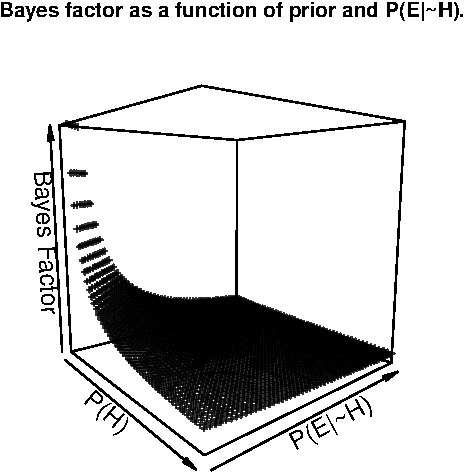
\includegraphics[width=1\linewidth]{lr-chapter4_files/figure-latex/fig-BayesFactorPrior-1} \end{center}
\caption{Impact of the prior and likelihood of E given ~H for probabilities in (0, 0.05) and Bayes Factor restricted to (0, 250) for visibility.}
\label{fig:BayesFactorPrior}
\end{figure}

A second reason to worry about the Bayes factor is its complexity. To
see this, the catch-all alternative hypothesis \(\neg H\) in the
denominator can be replaced by a more fine-grained set of alternatives,
\(H_1, H_2, \dots H_k\), provided \(H\) and these alternatives are
exclusive and cover the entire space of possibilities (that is, they
form a partition). The denominator becomes:
\begin{align} \label{eq:lotpLong}
\pr{E} & = \pr{E\vert H}\pr{H} +\sum_{i=1}^k \pr{E\vert H_i}\pr{H_i}. 
\end{align}

\noindent Estimating \(\pr{E}\) now looks quite difficult. It would
require one to sift through the entire space of possibilities, as well
as coming up with a sensible selection of priors probabilities for the
several alternative hypotheses on hand. Whoever is tasked with assessing
the strength of evidence---lay jurors, judges, or expert
witnesses---might face too great a cognitive burden.

A third reason to hesitate about the Bayes factor comes from an
observation by Gillies (1986), also discussed by Branden Fitelson
(1999). Consider the hypothesis \(H =\) ``the suspect is guilty'' and
suppose it is a fact that \(E =\) ``the suspect killed the victim.''
Fact \(E\) does not establish guilt with certainty since guilt requires
both \emph{actus reus}, the killing, and \emph{mens rea}, the intention.
But clearly \(E\) provides positive support for \(H\). Now consider a
composite hypothesis \(H'=\) ``the suspect is guilty \textit{and} we
live in a simulation built by aliens.'' Presumably, the support \(E\)
provides for \(H'\) should be weaker than the support it provides for
\(H\). After all, the addition of a far-fetched hypothesis should weaken
evidential support. This weakening, however, cannot be captured by the
Bayes factor since both \(H\) and \(H'\) deductively entail \(E\). In
general, suppose \(H\models E\) (and so, also, \(H \et X \models E\)).
Then both \(\pr{E\vert H}\) and \(\pr{E \vert H \et X}\) equal 1. But
this means that
\(\mathsf{BF}(H,E) = \mathsf{BF}(H \et X, E) = \nicefrac{1}{\pr{E}}\).
So the Bayes factors for the two support relations are equal. This is
the problem of irrelevant conjuncts.\footnote{The same point can be made
  using irrelevant hypotheses that are not so far-fetched. For instance,
  suppose one hypothesis of interest is whether the victim was running
  in the park on a certain night, and the relevant piece of evidence is
  her footprints in the park. Perhaps, another hypothesis is whether she
  had wine at dinner later on. Clearly, whether she did is not obviously
  relevant to whether she was running in the park beforehand. However,
  one should be very hesitant to say that the evidential strength of the
  presence of footprints is the same relative to
  \emph{she was running in the park} and
  \emph{she was running in the park and had wine at dinner later on}.
  But this is what the Bayes factor would commit one to.}

So suppose we are after a measure of evidential stregth that (i) does
not depend on priors, (ii) places no unreasonably heavy cognitive
requirements, and (iii) is sensitive to the addition of irrelevant
conjuncts. We will argue that a measure that satisfies these desiderata
is the likelihood ratio, the ratio between \(\pr{E \vert H}\) (the
probability of the evidence given the hypothesis is true) and
\(\pr{E \vert \neg H}\) (the probability of the evidence given the
hypothesis is false). Before showing that this measure satisfies the
three desiderata, we address a preliminary question. Why use such a
ratio in the first place?

For one thing, \(\pr{E \vert H}\) by itself is not fine-grained enough.
In some cases, this conditional probability may be close to one. For
instance, the probability that the blood from the crime matches the
accused, if the accused is the source,
\(\pr{\textsf{blood match} \vert \textsf{source}}\), may be close to
one. Similarly, the probability that the DNA from the crime scene
matches the accused, if the accused is the source,
\(\pr{\textsf{DNA match} \vert \textsf{source}}\), may also be close to
one. A quantity such as \(\pr{E \vert H}\), by itself, would make no
distinction here, but a DNA match is not on par with a blood type match.
The DNA match should be stronger incriminating evidence than the blood
type match because a specific DNA profile typically is less common than
a specific blood type. This difference can be captured by the other
conditional probability \(\pr{E \vert \neg H}\). If the accused is
\textit{not} the source, the probability of a blood type match, while
relatively small, should be higher than the probability of a DNA profile
match. Consequently, the likelihood ratio for the DNA match would be
higher than that for the blood match, as expected.\footnote{Specifically,
  \(\nicefrac{\pr{\textsf{DNA match} \vert \textsf{source}}}{\pr{\textsf{DNA match} \vert \neg \textsf{source}}} > \nicefrac{\pr{\textsf{blood match} \vert \textsf{source}}}{\pr{\textsf{blood match} \vert \neg \textsf{source}}}\).}

For similar reasons, the strength of evidence cannot be measured by the
probability \(\pr{E \vert \neg H}\) alone. Consider an example by Triggs
\& Buckleton (2004). In a child abuse case, the prosecutor offers
\label{text:rock} evidence that a couple's child rocks and that only 3\%
of non-abused children rock,
\(\pr{\textsf{child rocks} \vert \neg \textsf{abuse}}=.3\). If it is
unlikely that a child who is not abused would rock, that this child
rocks might seem evidence of abuse. But this interpretation is mistaken.
It could also be that 3\% of abused children rock,
\(\pr{\textsf{child rocks} \vert \textsf{abuse}}=.3\). After all, the
two conditional probabilities need not add up to one. If rocking is
equally unlikely under either hypothesis, rocking cannot count as
evidence of abuse.

So, both the probability of the evidence given the hypothesis and the
probability of the evidence given an alternative hypothesis should be
part of any good measure of evidential strength (ENFSI, 2015; Royall,
1997; Triggs \& Buckleton, 2004). The Bayes factor includes both
probabilities, but---as seen before---it falls prey to several
difficulties. A more promising measure is the \textbf{likelihood ratio}:
\begin{align}
\label{eq:LR}
\tag{LR}
\mathsf{LR}(E,H,H') & = \frac{\pr{E \vert H}}{\pr{E \vert H'}},
\end{align}

\noindent where \(H'\) is a hypothesis that is taken to be a competing
alternative to \(H\). If the evidence is more likely given \(H\) than
\(H'\), the ratio would be above one, and if the evidence is more likely
given \(H'\) than \(H\), the ratio would be below one. As with the Bayes
factor, support levels correspond to deviations from one. The greater
the likelihood ratio (for values above one), the stronger the evidence
in favor of \(H\) as contrasted with \(H'\). The smaller the likelihood
ratio (for values below one), the stronger the evidence in favor of the
competing hypothesis \(H'\) as contrasted with \(H\).

Its simplicity makes the likelihood ratio well-suited for presentation
in trial proceedings. An expert, for instance, may testify that the
blood-staining on the jacket of the defendant is ten times more likely
to be seen if the wearer of the jacket hit the victim (prosecutor's
hypothesis) rather than if he did not (defense's hypothesis) (CGG
Aitken, Roberts, \& Jackson, 2010, p. 38). This apparent simplicity,
however, can give rise to confusions in the assessment of the evidence,
especially if the hypotheses are not stated clearly. In the most
straightforward case, \(H'\) is just the negation of \(H\). But the
competing hypotheses \(H\) and \(H'\) need not be one the negation of
the other, a point to which we will return.

Let's now examine why the likelihood ratio satisfies our three
desiderata. First, unlike the Bayes factor, the likelihood ratio does
not depend on the prior probability of the hypothesis. The relationship
between likelihood ratio, prior and posterior odds is apparent in the
odds version of Bayes' theorem: \begin{align}\label{eq:BTodds}
\frac{\pr{H \vert E}}{\pr{H' \vert E}}= \frac{\pr{E \vert H}}{\pr{E \vert H'}}\times \frac{\pr{H}}{\pr{H'}}.
\end{align} \noindent If the likelihood ratio is greater (lower) than
one, the posterior odds will be greater (lower) than the prior odds of
\(H\). The likelihood ratio, then, is a measure of the upward or
downward impact of the evidence on the prior odds of two hypotheses
\(H\) and \(H'\).\footnote{The meaning of the likelihood ratio can be
  made more perspicuous by supplementing it with a graph that conveys
  visually the extent to which the evidence changes the probability of
  the hypothesis of interest (See Figure \ref{fig:effect-evidence}).}
This fits nicely with the division of labor common in legal fact-finding
between experts and decision-makers, judges or lay jurors. A prominent
forensic scientist recommends that `in criminal adjudication, the values
of the prior odds and the posterior odds are matters for the judge and
jury, in accordance with the normal division of labor in forensic
fact-finding' (Colin Aitken \& Taroni, 2008, p. 194). Other scholars
reccomend that experts should `not trespass on the province of the jury
by commenting directly on the accused's guilt or innocence, \dots and
should generally confine their testimony to presenting the likelihood of
their evidence under competing propositions' (CGG Aitken, Roberts, \&
Jackson, 2010, p. 42).

\begin{figure}[h]

\begin{center}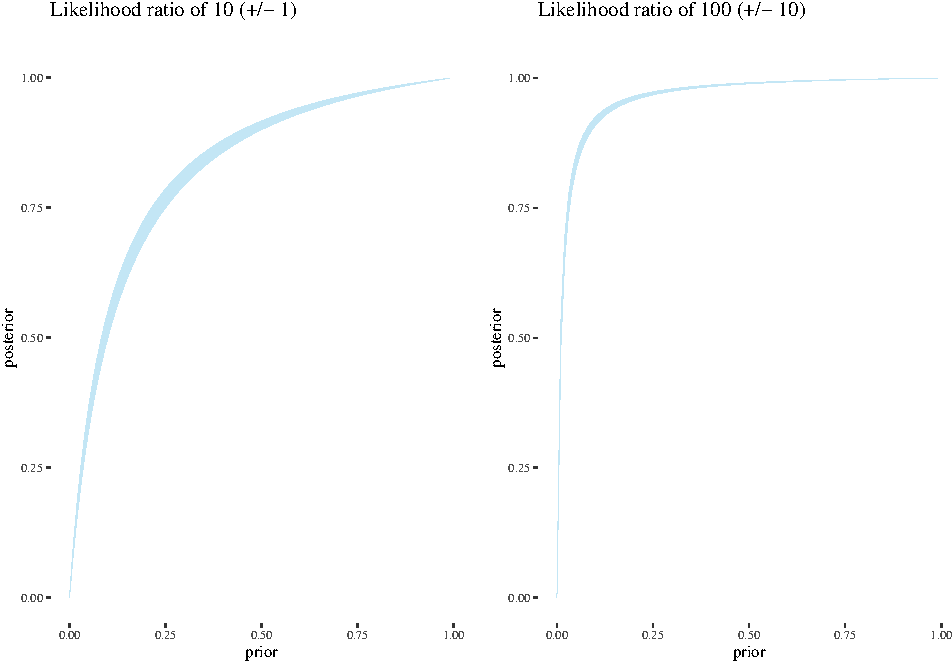
\includegraphics[width=1\linewidth]{lr-chapter4_files/figure-latex/effect-evidence-b-1} \end{center}
\caption{This graphical representation can supplement the likelihood ratio to convey visually the extent to which the evidence changes the probability of the hypothesis. This representation assumes that the two hypotheses in the likelihood ratio are one the negation of the other. In this case, the posterior probability of $H$ equals $\nicefrac{PO}{1+PO}$, where $PO$ are the posterior odds.}
\label{fig:effect-evidence}
\end{figure}

Second, the likelihood ratio is less cognitively burdensome than the
Bayes factor. It does not require one to think about the probability of
the evidence in general, \(\pr{E}\). Think, for example, of blood match
evidence. To calculate the Bayes factor, we need two things:
\(\pr{E\vert H}\) (which here, say, can be assumed to approximate one)
and \(\pr{E}\) (which is the probability of a blood match under any
possible scenarios, whether or not the the suspect is the source). Yet,
direct and reliable estimation of the probability \(\pr{E}\) is
difficult. One can use the law of total probability from equation
\eqref{eq:lotpSimple}. This would require, besides an assessment of the
conditional probabilities \(\pr{E\vert H}\) and \(\pr{E\vert \neg H}\),
an assessment of the prior probabilities of \(\pr{H}\) and
\(\pr{\neg H}\). Instead, the likelihood ratio would only require an
assessment of the conditional probabilities. In this sense, its
calculation requires less information.

Finally, unlike the Bayes factor, the likelihood ratio is not
susceptible to the problem of irrelevant hypotheses. For suppose
\(\pr{E\vert H} = \pr{E\vert H \et X} = 1\), where \(X\) is an
additional hypothesis that is irrelevant to \(H\). Note that
\(\mathsf{LR}(E,H) = \nicefrac{1}{\pr{E \vert \n H}}\), while
\(\mathsf{LR}(E, H \et X) = \nicefrac{1}{\pr{E \vert \n H \vee \n X}}\).
Unlike with the Bayes factor, here the two denominators might differ.
For example, suppose a fair coin is tossed three times. Let \(H=\) ``two
first tosses resulted in two heads,'' let \(E=\) ``at least one of the
two first tosses resulted in a head,'' and let \(X=\) ``the third toss
resulted in heads.'' Then \(\pr{E \vert H} =1\),
\(\pr{E\vert \n H} = \nicefrac{2}{3}\),
\(\mathsf{LR}(E,H) = \frac{1}{\nicefrac{2}{3}} = 1.5\). However,
\(\pr{E\vert H \et X} =1\), \(\pr{E \vert \n (H \et X)} \approx .71\),
so \(\mathsf{LR}(E,H \et X) \approx \frac{1}{.71} = 1.4\). Thus, the
support, as measured by the likelihood ratio, can drop by adding a
conjunct that is probabilistically irrelevant to the original
hypothesis. In fact, this weakening of evidential support by adding an
irrelevant conjunct holds in general for the likelihood ratio given
sensible assumptions.\footnote{Branden Fitelson (2002) proved a general
  claim about irrelevant conjunctions. Hawthorne \& Fitelson (2004)
  later strengthened this claim. The claim is that, if
  \(\mathsf{LR}(E,H,\n H)>1\),
  \(\pr{E \vert X \et H} = \pr{E \vert H}\), and
  \(\pr{X \vert H} \neq 1\), then
  \(\mathsf{LR}(E,H,\n H) > \mathsf{LR}(E,H \et X,\n(H \et X))\). Crupi
  \& Tentori (2010) raised a related problem. They point out that if
  \(\mathsf{LR}(E,H)\leq 1\) and \(X\) is confirmationally irrelevant
  conjunct to \(H\) with regard to \(E\), then \(E\) will have the same
  negative or null impact on \(H \et X\), that is
  \(\mathsf{LR}(E,H \et X ) \leq \mathsf{LR}(E,H)\). They find this
  counter-intuitive and argue that this can be avoided by switching to
  the \(\mathsf{Z}\) confirmation measure (Crupi, Tentori, \& Gonzalez,
  2007). As we argue in Appendix \ref{sec:confirmation}, the
  \(\mathsf{Z}\) measure is prior-sensitive and therefore not fit for
  our purpose. Further, the phenomenon might not be deeply troubling
  either. If the likelihood ratio tracks how strongly the evidence
  supports a hypothesis, it should be no surprise that a more complex
  hypothesis---one obtained by adding an irrelevant
  proposition----enjoys a lower support from the same evidence.}

\vspace{1mm}
\footnotesize

\normalsize

All in all, the likelihood ratio outperforms the Bayes factor on several
respects. But, of course, there could be other measures of evidential
strength that fare even better. Other measures worth considering come
from the literature in formal epistemology on confirmation theory. The
expression `confirmation' is more common in this literature than
`strength' (or value, support). A discussion of these measures, however,
would detract us from the main task at hand. We therefore relegate it to
Appendix \ref{sec:confirmation}. In it, we argue that two questions
should be distinguished. (1) To what extend does a piece of evidence
change our beliefs about a given hypothesis? (2) What is the strength
(value, support) of a piece of evidence relative to a hypothesis? The
two questions overlap to some extent. But the difference is that
confirmation depends on prior probabilities, while evidential strength
should be kept separate from prior probabilities. Confirmation measures
are concerned with (1) rather than (2), and thus they are unsuitable for
the evaluation of evidence in trial proceedings.

\hypertarget{match-evidence-and-error-probabilities}{%
\section{\texorpdfstring{Match evidence and error probabilities
\label{sec:fp}}{Match evidence and error probabilities }}\label{match-evidence-and-error-probabilities}}

The two conditional probabilities that make up the likelihood
ratio---\(\pr{E \vert H}\) and \(\pr{E \vert \neg H}\)---should be used
in the evaluation of any form of evidence, both quantitative and
non-quantitative. This section examines how a DNA match, a widely used
form of quantitative evidence, should be evaluated by means of the
likelihood ratio. The argument formulated here can be generalized to any
`match evidence.' The match can be between genetic profiles,
fingerprints, blood types, bite marks, etc.

Consider an expert testimony that there is a genetic, DNA match between
the traces at the crime scene and a sample from the defendant. This
statement is evidence that the defendant was the \textit{source} of the
traces---that the materials found at the scene originated from the
defendant. The match can also be evidence that the defendant was present
at the scene or committed the crime, but these claims are more
questionable, as the chain of inferences is weaker. For simplicity, let
us focus on the source hypothesis. The likelihood ratio we should be
concerned with is therefore the following:
\[\frac{\pr{\textsf{match} \vert \textsf{source}}}{\pr{\textsf{match} \vert \neg \textsf{source}}}.\]

\noindent How strongly does a match favor the source hypothesis? To
answer this question, the simplest analysis relies on the
\textbf{random match probability}, the probability that a random person,
unrelated to the crime, would coincidentally match the crime scene
profile. When experts testify about a DNA match, they often only provide
the random match probability as an indicator of evidential strength.
This probability coincides (roughly) with the denominator of the
likelihood ratio, that is, the probability that someone who is not the
source would match. What about the numerator? The assumption often made
is that the numerator is close to one. Since the random match
probability is usually an impressively low number, say 1 in 100 million,
this is enough to ensure that the likelihood ratio is significantly
above one.

This analysis, though simple and elegant, lacks precision in at least
two respects. First, it assumes that the numerator
\(\pr{\textsf{match} \vert \textsf{source}}\) is close to one. But a DNA
match need not track with 100\% probability the fact that the suspect is
the source. There could be false negative matches. In addition---and
more importantly---equating the denominator
\(\pr{\textsf{match} \vert \neg \textsf{source}}\) with the random match
probability ignores the risk of false positive matches. This risk is not
negligible (Shaer, 2016). The denominator, then, should depend on two
sources of error: a false positive match and a coincidental match. These
errors are quite distinct. For suppose two individuals---say the
perpetrator and the defendant---happen to share the same DNA profile by
coincidence. If an expert states that the crime scene sample and the
defendant's sample match, this would be a coincidental match, not a
false positive match. This risk of error is captured by the random match
probability. But if the two samples do not actually match, and yet the
expert says that they do, this would count as a false positive match,
not a coincidental match. This risk of error is not captured by the
random match probability.

Unlike a coincidental match, a false positive match is often caused by a
human error in a number of circumstances (see W. C. Thompson, 2013 for a
more exhaustive treatment and multiple examples):

\raf{A: Bib references are missing here, is it on purpose?}

\begin{itemize}
\item
  \textbf{Cross-contamination of samples.} For instance, in Dwayne
  Johnson (2003) samples were accidentally swapped. In Lukis Anderson
  (2012), the genetic material was carried over by the paramedics. In
  one case, German police invested a considerable amount of time and
  effort searching for the so-called Phantom of Heilbronn, whose DNA
  profile was associated with many crimes. A bounty of EUR 300,000 was
  placed on her head. It turned out she was an innocent employee
  involved in the production of cotton swabs used across the country.
\item
  \textbf{Mislabeling of samples.} For instance, in 2011 the Las Vegas
  Metropolitan Police Department acknowledged that samples of two men
  suspected of a 2001 robbery were switched, leading to the exclusion of
  the perpetrator and four years of incarceration for the other suspect.
  The mistake came to light only because the perpetrator was later
  arrested for another crime.
\item
  \textbf{Misinterpretation of test results.} Single-source sample
  comparison is not easily prone to misrepresentation, but evidence
  mixtures---often needed in sexual assault cases---are complicated to
  interpret. For example, Dror \& Hampikian (2011) re-examined a 2002
  Georgia rape trial in which two forensic scientists had concluded that
  the defendant could not be excluded as a contributor of the crime
  traces. The evidence was sent to 17 lab technicians for
  re-examination. One of them agreed that the defendant could not be
  excluded as a contributor. Twelve considered the DNA exclusionary, and
  four found it inconclusive. If the quantity of DNA is limited, there
  is uncertainty about the number of contributors and about whether any
  alleles are missing. Ultimately, there is an element of subjectivity
  in mixed DNA interpretation.
\end{itemize}

\begin{center}
\begin{figure}
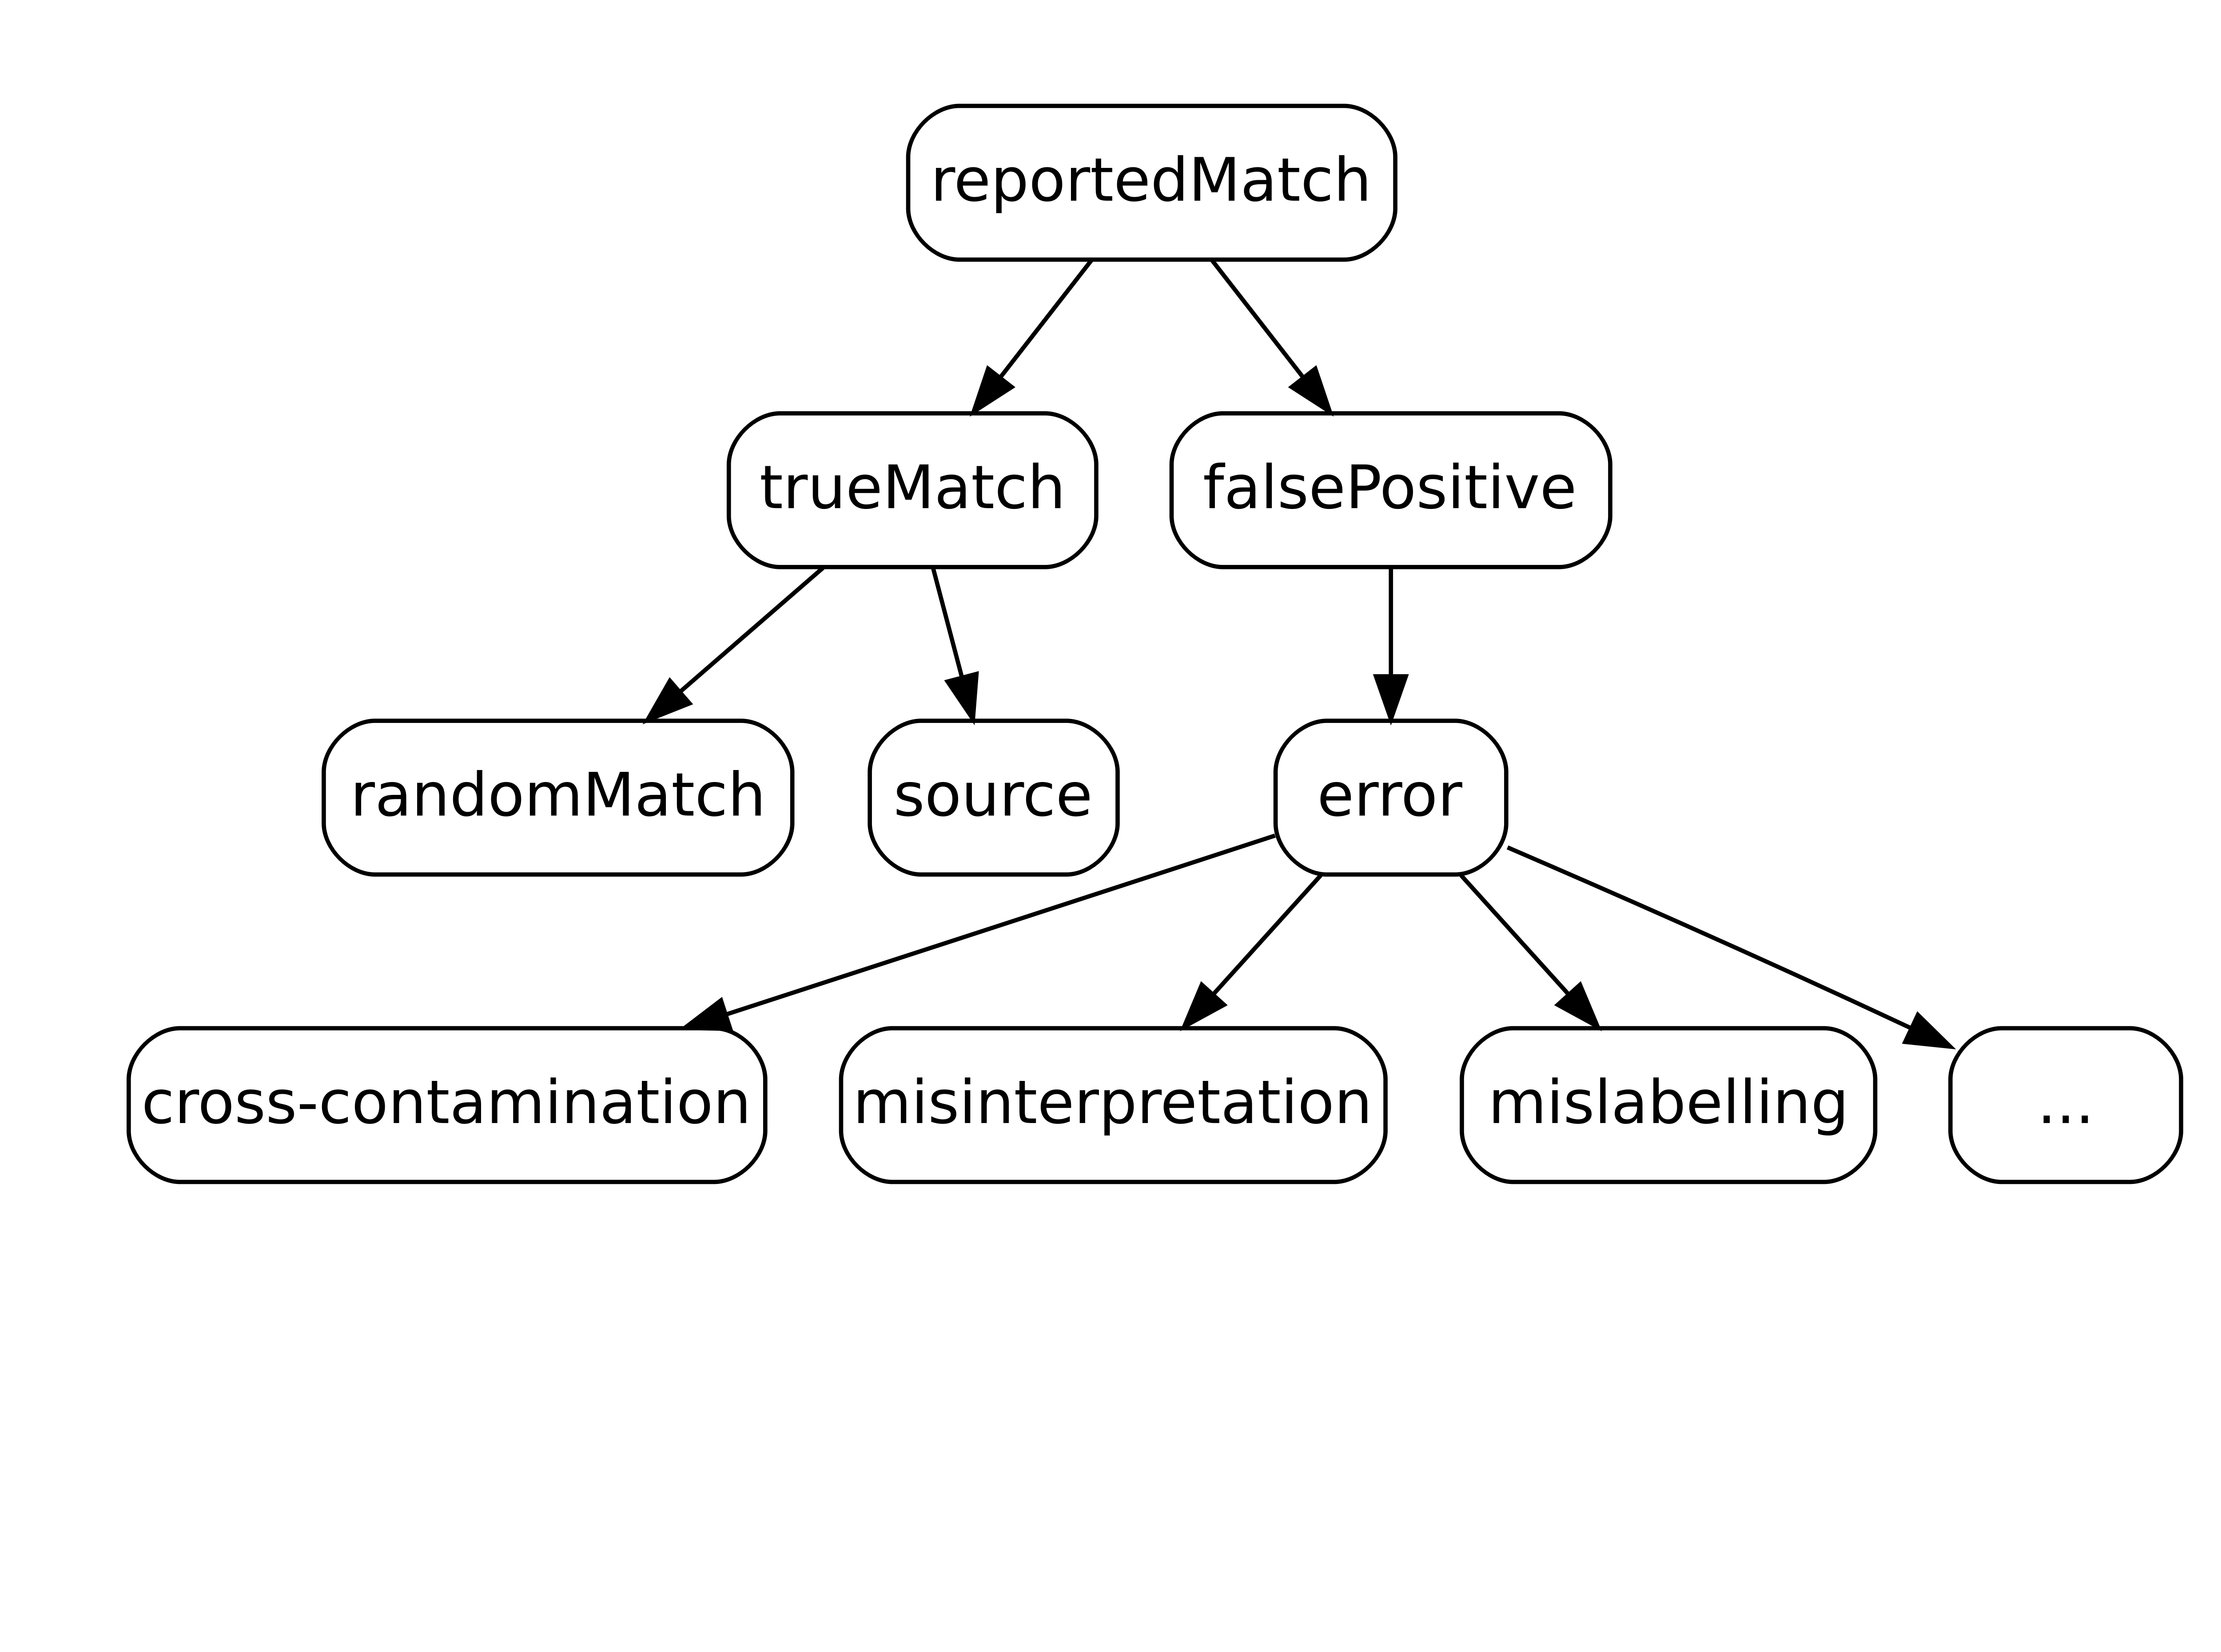
\includegraphics[width = 12cm]{img/fpp.png}
\caption{Dependencies between variables in the false positive problem.}
\label{fig:fpp}
\end{figure}
\end{center}

So, a careful analysis should take into account the risks of false
positive and false negative matches in the assessment of DNA evidence
This can be done using the likelihood ratio, following Colin Aitken,
Taroni, \& Thompson (2003). False positives are usually more worrisome
than false negatives as they increase the risk of a mistaken conviction.
That is also why we devoted to them more space in the foregoing
discussion. But, for the sake of completeness, we will consider both.

This more refined analysis begins by making a conceptual distinction
between true match and reported match. A true match is the fact that two
samples actually carry the same genetic profile, while a reported match
is a statement made by an expert that two samples match. A true match
will exist not only if the suspect is the source, but also if, even
though the suspect is not the source, the profiles are in fact the same
due to a random, coincidental match. Similarly, a reported match might
arise not only if there is a true match, but also if a false positive
error has been made. These possibilities are represented in Figure
\ref{fig:fpp}. For ease of reference, we will use the following
abbreviations:

\begin{center} \hspace{10mm}
\begin{tabular}{lp{9cm}}
$S$ & The specimen comes from the suspect (source). \\
$R$ & A match is reported (reported match). \\
$M$ & There is a true match (true match).
\end{tabular}
\end{center}

\noindent  In this set-up, the evidence to be assessed is the
\textit{reported} match relative to the pair of hypotheses \(S\) and
\(\neg S\). So the likelihood ratio we are after has the form:
\[\frac{\pr{R \vert S}}{\pr{R \vert \neg S}}.\]

\noindent With a few manipulations and assumptions in place, the
likelihood ratio can be written as:\footnote{By the law of total
  probability, the denominator \(\pr{R \vert \neg S}\) can be unpacked
  as \(\pr{R \wedge M \vert \neg S} + \pr{R \wedge \neg M | \neg S}\).
  The latter, by the chain rule, is equivalent to
  \(\pr{R \vert M \wedge \neg S}\pr{ M \vert \n S} + \pr{R \vert \n M \wedge \neg S}\pr{\n M \vert \n S}\).
  A similar reasoning applies to the numerator. So we have:
  \[\frac{\pr{R \vert S}}{\pr{R \vert \neg S}} = \frac{\pr{R \vert M \et S}\pr{M \vert S} + \pr{R \vert \n M \et S}\pr{\n M \vert S}} {\pr{R \vert M \et \n S}\pr{M \vert \n S} + \pr{R \vert \n M \et \n S}\pr{\n M \vert \n S}}
  \] Both numerator and denominator can be simplified because a reported
  match (\(R\)), given a true match obtains (\(M\)), is independent of
  whether the suspect is the source (\(S\)):
  \[\pr{R \vert M \et S} = \pr{R \vert M \et \n S} = \pr{R \vert M}\]
  \[\pr{R \vert \n M \et S} = \pr{R \vert\n M \et \n S} = \pr{R \vert \n M}\]
  Finally, in the numerator, let the probability of a true match if the
  suspect is the source be one:
  \[\pr{M\vert S} = 1  \,\,\, \mbox{ so also } \,\,\, \pr{\n M \vert S}=0.\]
  This assumption holds in virtue of the meaning of the statements
  involved. That the suspect is the source of the crime sample entails,
  almost analytically, that the two samples must carry the same genetic
  profile.} \begin{align}
\label{eq:LRfp4}
\frac{\pr{R \vert S}}{\pr{R \vert \neg S}} & = \frac{
\pr{R \vert M}
}{
\pr{R \vert M }\pr{M \vert \n S} +
\pr{R \vert \n M}\pr{\n M \vert \n S}
}
\end{align}

\noindent Note that, as intended, the numerator \(\pr{R \vert M}\) can
be different from one, since a false negative reported match can occur
(or, which is the same, a true match need not always occur). The
denominator reflects the fact that there are two ways misleading
evidence can arise: there is a true match and the suspect is not the
source (because of a random, coincidental match), or there is no true
match, and a false positive error has been made in the identification
process.

To make the different sources of error more salient---false negative
matches, false positive matches and random or coincidental matches---the
likelihood ratio can be written, as follows:

\begin{align}
\label{eq:LRfp4b}
\frac{\pr{R \vert S}}{\pr{R \vert \neg S}} & = \frac{1-FNP}{[(1-FNP)\times RMP] + [ FPP \times (1-RMP)]}
\end{align}

\noindent This is the same as the formula above. The expression FNP
stands for the false negative probability \(\pr{\neg R \vert M}\), so
\(1-FNP\) equals the true positive probability \(\pr{R \vert M}\). The
expression FPP stands for the false positive probability
\(\pr{R \vert \n M}\). The expression RMP stands for the random match
probability \(\pr{M\vert \n S}\). A false positive or false negative
probability track a human error, the possibility that a match may be
reported (\(R\)) even without a true match (\(\neg M\)) or that a match
may \textit{not} be reported (\(\neg R\)) even with a true match
(\(M\)). The random match probability, instead, tracks a coincidence of
nature, the possibility that someone who is not the source (\(\neg S\))
could still be---coincidentally---a true match (\(M\)).

Let's now examine the impact of the error probabilities FNP and FPP on
the likelihood ratio, holding fixed certain values of the random match
probability. Figure \ref{fig:fpplr} shows the impact of the false
positive probability FPP (for values between 0 and .05) while the false
negative probability FNP is kept to zero. Random match probabilities are
assumed to be in the order of \(10^{-9}\) (often reported in the case of
two single-source samples over ten or more loci) and \(10^{-3}\)
(sometimes obtained by means of less discriminating tests when the
comparison involves a mixed sample). A small increase in the false
positive probability can lower the likelihood ratio dramatically.
Interestingly, however, the impact of the false negative probability FNP
(for values between 0 and .05) is negligible, as shown in Figure
\ref{fig:fpfnplr}.

\begin{figure}

\begin{center}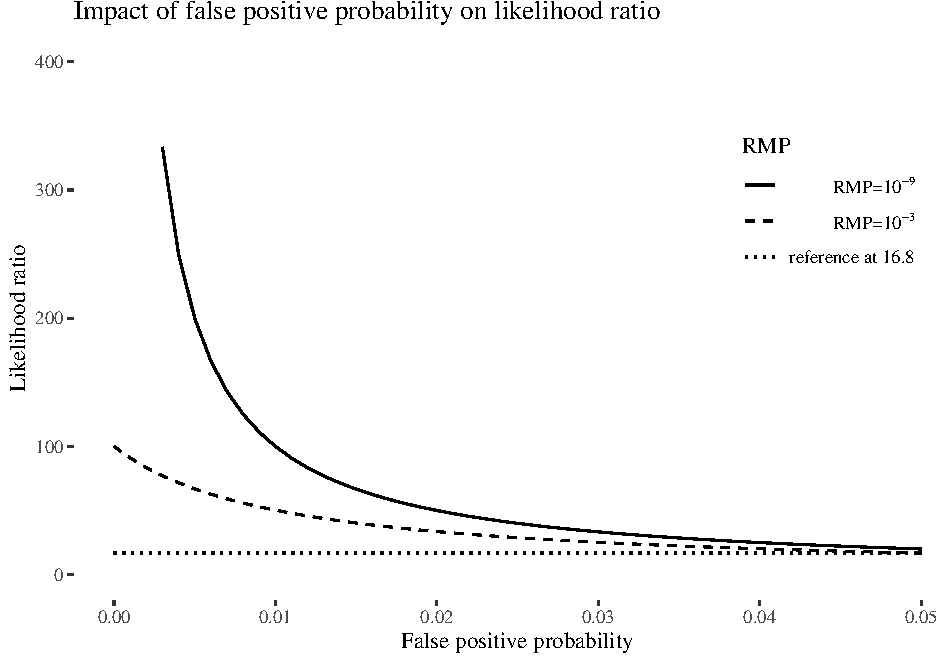
\includegraphics[width=1\linewidth]{lr-chapter4_files/figure-latex/fig-fpplr-1} \end{center}
\caption{Positive match: Impact of the false positive probability on the likelihood ratio for two values of RMP. The horizontal reference line is at 16.8, the likelihood reached at RMP=$10{^-3}$ for FPP=0.05. At the same value of FPP, the LR for RMP $10{^-9}$ is 20.}
\label{fig:fpplr}
\end{figure}

\begin{figure}

\begin{center}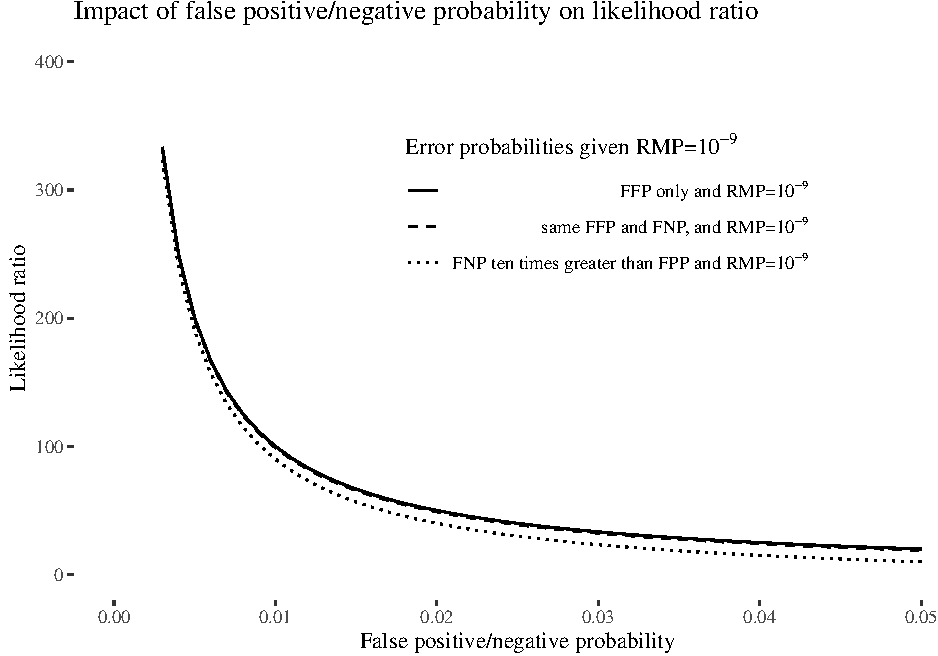
\includegraphics[width=1\linewidth]{lr-chapter4_files/figure-latex/fig-fpfnplr-1} \end{center}
\caption{Positive match: impact of the false positive probability FPP and false negative probability FNP on the likelihood ratio, assuming RMP=$10{^-9}$. For simplicity, the two error probabilities are assumed to be the same. The impact of FNP is negligible.}
\label{fig:fpfnplr}
\end{figure}

A similar analysis can be used to study the impact of error
probabilities on the value of exculpatory DNA evidence, corresponding to
a \textit{negative} (reported) match \(\neg R\). By replacing \(R\) with
\(\neg R\) in formula (\ref{eq:LRfp4}), the likelihood ratio becomes:
\begin{align}
\label{eq:LR-match-exc}
\frac{\pr{\neg R \vert S}}{\pr{\neg R \vert \neg S}} & = 
\frac{\pr{\neg R \vert M}}{\pr{\neg R \vert M }\pr{M \vert \n S} + \pr{\neg R \vert \n M}\pr{\n M \vert \n S}}\\
& = \frac{FNP}{FNP\times RMP + [(1-FPP) \times (1-RMP)]}
\end{align}

\noindent Keep in mind that the negative reported match \(\neg R\) is
evidence \textit{against} the source hypothesis \(S\) so long as the
likelihood ratio is below one. At the extreme, if the false negative
probability FNP is zero, the numerator is zero. Thus, the likelihood
ratio will be zero, as it should. In such a case, the negative match is
completely exculpatory, and the posterior probability that the suspect
is the source will also be zero. If the false negative probability is
not zero, the greater the likelihood ratio (for values between 0 and 1),
the weaker the value of the exculpatory match. As Figure
\ref{fig:fpfnplr-exc} shows, the likelihood ratio progressively moves
away from zero as the false negative error probability increases.
Interestingly, however, the impact of the false \textit{positive}
probability FPP on the likelihood ratio of exculpatory evidence is
essentially null.

\begin{figure}[t]

\begin{center}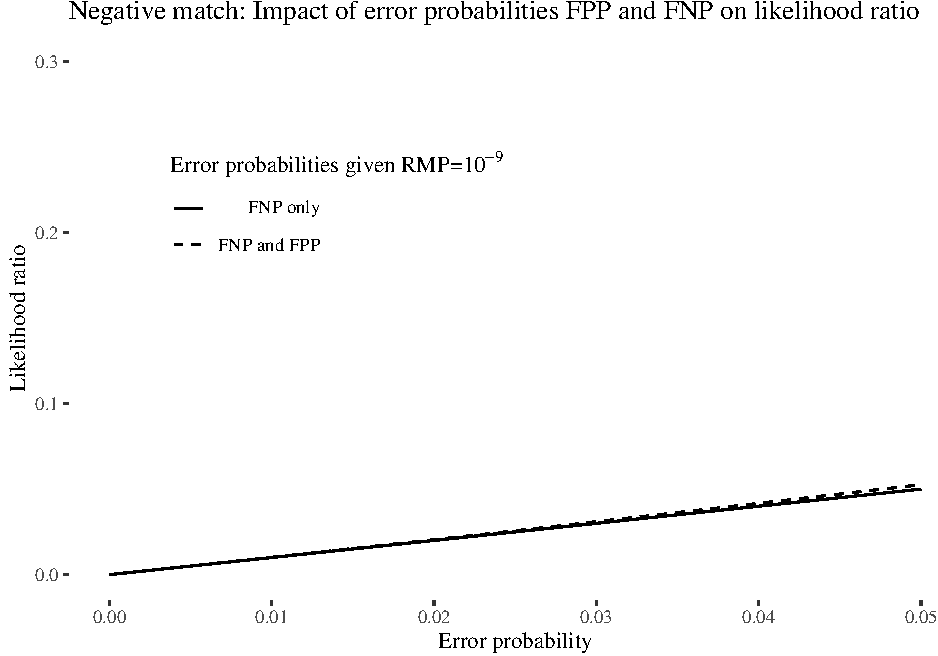
\includegraphics[width=1\linewidth]{lr-chapter4_files/figure-latex/fig-fpfnplr-exc-1} \end{center}
\caption{Negative (exculpatory) DNA match. Impact of the false positive probability FPP and false negative probability FNP on the likelihood ratio, assuming a RMP=$10{^-9}$. For simplicity, the two error probabilities are assumed to be the same. The impact of FPP is negligible.}
\label{fig:fpfnplr-exc}
\end{figure}

\begin{figure}[h]

\begin{center}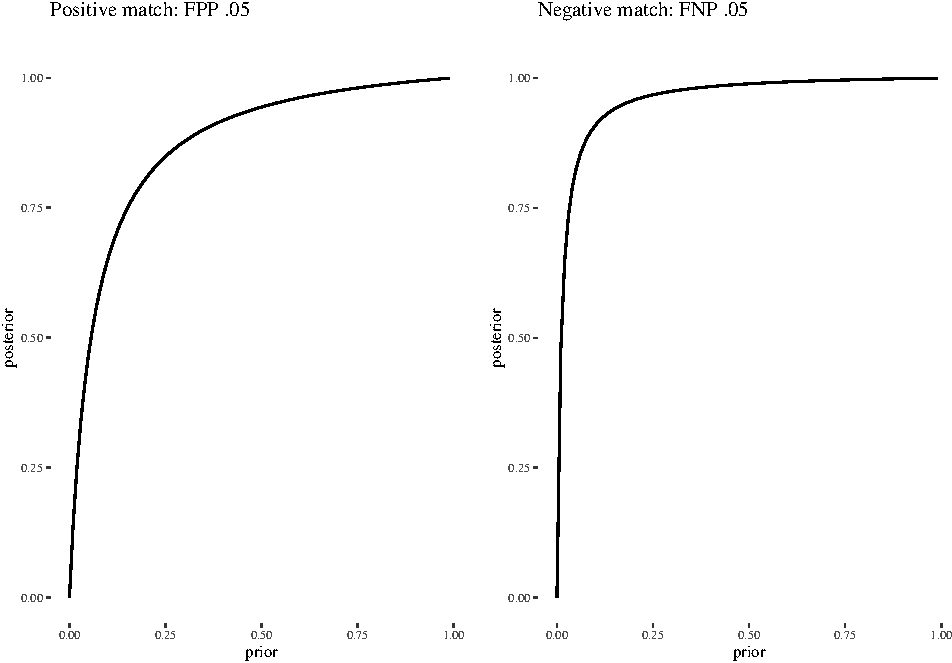
\includegraphics[width=1\linewidth]{lr-chapter4_files/figure-latex/ex-inc-dna-b-1} \end{center}
\caption{How positive and negative matches, subject to the same error probability, affect the probability of the source hypothesis.}
\label{fig:ex-inc-dna}
\end{figure}

\raf{M: Right graph in Figure \ref{fig:ex-inc-dna}is wrong, but when you compile the individual chunk, the graph come sout corerect. Mystery!}

So, even a seemingly small error probability trumps the random match
probability. If there are good reasons to worry about random matches,
there are even better reasons to worry about error probabilities. In
addition, this analysis shows which error probabilities we should be
concerned about and in which circumstances. The impact of the error
probabilities is not uniform, contrary to what one might intuitively
think. The false positive probability has a marked impact on the value
of incriminating DNA evidence (positive matches), while the false
negative probability has a marked impact on the value of exculpatory DNA
evidence (negative matches).\footnote{The impact of false positive and
  false negative probabilities is not symmetric across positive and
  negative matches when evidential value is measured by the likelihood
  ratio. For positive matches, even a small false positive probability
  can cause the likelihood ratio to drop significantly, as Figure
  \ref{fig:fpplr} and \ref{fig:fpfnplr} show. Instead, for negative
  matches, Figure \ref{fig:fpfnplr-exc} shows that even a false negative
  probability as high as 5\% has a minor effect on the likelihood ratio,
  which remains relatively close to zero. But this asymmetry is just an
  artifact of using the likelihood ratio as a measure of evidential
  strength. Error probabilities for a positive or negative match affect
  the posterior probability of the source hypothesis equally strongly.
  For suppose the random match probability is \(10^{-3}\) and the prior
  probability of \(S\) is .5. Without taking into account the error
  probabilities, a positive match would bring the probability of \(S\)
  from .5 to .99. Instead, taking into account a false positive
  probability of 0.05, a positive match would bring the probability of
  \(S\) from .5 to just about .94. What about a negative match? Without
  taking into account the error probabilities, a negative match would
  bring the probability of \(S\) from .5 to 0. Instead, taking into
  account a false negative probability of 0.05, a negative match would
  bring the probability of \(S\) from .5 to just about .04. See, more
  generally, \ref{fig:ex-inc-dna}. Furthermore, a positive match
  followed by a negative match, each subject to the same error
  probabilities, would have no impact on the posterior probability of
  the source hypothesis. All in all, the likelihood ratio should be
  interpreted carefully, a point to which we will return later in this
  chapter.} Conversely, a false negative probability has a negligible
impact on the value of incriminating DNA evidence, while a false
positive probability has a negligible impact on the value of exculpatory
DNA evidence.

But, no doubt, these claims are still rather hypothetical.
Unfortunately, no serious attempt has been made to systematically
quantify the relevant error probabilities. Sometimes, a lab discovers
its own errors and reports them, but this is rare (W. C. Thompson,
2013). Anecdotal information suggest that false positive matches take
place more often than coincidental matches would entail, but how often
remains unclear (W. C. Thompson, 2013). Regular proficiency tests used
in accredited DNA laboratories involve comparison of samples from known
sources, but they are criticized for being unrealistically easy (yet, it
happens that analysts fail them). Sometimes, corrective action files are
made available. They usually show relatively few false positive
errors.\footnote{For instance, the Santa Clara County district
  attorney's crime laboratory between 2003 and 2007 caught 14 instances
  of evidence cross-contamination with staff DNA, three of contamination
  by unknown person, and six of DNA contamination from other samples,
  three cases of DNA sample switch, one mistake in which the analyst
  reported an incorrect result, and three errors in the computation of
  the statistics to be reported.} But because of the fragmentary data
available, it is premature to conclude there is no reason for concern.

More data should be collected to plug in the right values of false
positive and false negative probabilities in the likelihood ratio. These
error probabilities should be case-specific, not generic. After all, the
objective is to assess the risk of error for \textit{this} match, not a
match in general \todo{add references}. To this end, numerical data
should be collected that are fine-grained enough to document the error
probabilities, FPP and FNP, corresponding to scenarios in which specific
procedures, safeguards, or protocols are followed. As experts who
testify about a match (or lack thereof) are cross-examined at trial,
they will testify about the procedures, safeguards and protocols that
the laboratory technicians followed in the specific case. This
case-specific information could then be combined with performance data
about error probabilities under different scenarios. This would yield a
case-specific assessment of the value of match evidence.

We conclude this section by noting that other proposals exist in the
literature for formulating the likelihood ratio of a genetic match which
also incorporate error probabilities. Another, more general proposal is
due to Buckleton, Bright, \& Taylor (2018). But, interestingly, the
likelihood ratio of a DNA match used in equations (\ref{eq:LRfp4}) and
(\ref{eq:LR-match-exc}) turns out to be a particular case of this more
general approach. This convergence is encouraging. Here we briefly go
through the derivation.

First, Buckleton and co-authors make the conceptual distinction between
the probability that an error occurs, \(\pr{ERR}\), and the probability
that a match is reported if an error occurs, \(\pr{R \vert ERR}\). Let
\(err\) denote the probability of error, and we assume it to be
independent of the source hypothesis:\\
\begin{align*}
err & = \pr{ERR} = \pr{ERR \vert S} = \pr{ERR \vert \n S}
\end{align*} \noindent 
\raf{M: I don't see why this independence holds. Can you explain?}
Separately, let \(k\) denote the probability of a reported match if an
error occurs, also assumed to be independent of whether the source
hypothesis is true: \begin{align*}
k & = \pr{R \vert ERR} = \pr{R \vert ERR, S} = \pr{R \vert ERR, \n S}
\end{align*} \noindent  Now the derivation: \begin{align*}
LR & = \frac{\pr{R\vert S}}
{\pr{R \vert \n S}}\\
& = \frac{\pr{R \vert \n ERR, S}\pr{\n ERR \vert S} + \pr{R \vert ERR, S}\pr{ERR \vert S}}
{\pr{R \vert \n ERR, \n S}\pr {\n ERR \vert \n S} + \pr{R \vert ERR, \n S}\pr{ERR \vert \n S}}\\
& = \frac{1\times (1-err) + k\times err}
{RMP\times (1-err)+k\times err}  = \frac{1-err+k\times err}{RMP  - err\times RMP + k \times err} \\
& = \frac{1 - (1-k)err}{RMP\times (1-err)+k\times err}
\end{align*} \noindent As before, the likelihood ratio is the ratio of
the probabilities of a reported match if the suspect is the source and
if the suspect is not the source. The numerator \(\pr{R\vert S}\) can be
split into two possible scenarios: an error has not been made, or an
error has been made. Accordingly, the numerator in the second line uses
the law of total probability to split \(\pr{R\vert S}\) into these two
options. Similarly, the numerator \(\pr{R\vert \n S}\) can be split into
two cases: the suspect is not the source, but we are dealing with a
random match, or the suspect is not the source, and an error has been
made. An application of the law of total probability in the denominator
mirrors this. The rest of the argument is just rewriting in terms of
abbreviations, and algebraic manipulation. The probability of a reported
match \(R\) if no error occurs \textit{and} the source hypothesis is
false is the random match probability RMP, so
\(\pr{R \vert \n ERR, \n S}=RMP\). The probability that a reported match
occurs when the source hypothesis is true and no error has made is
assumed to be one, so \(\pr{R \vert S, \n ERR} =1\).

\todo{this bit still needs polishing}

Finally, if you think of an error as something that guarantees a
mistaken reported match, \(k\) becomes \(1\) and \(e\) becomes the false
positive rate. On this assumption straightforward algebraic manipulation
gives: \begin{align*}
 \frac{1 - (1-k)\times err}{RMP\times (1-err)+k\times err} & = \frac{1-err+err}{RMP(1-err)+err}\\
 & = \frac{1}{RMP - err\times RMP + err} = \frac{1}{1 + err\times(1-RMP)}
\end{align*} \noindent which is the same as the formula obtained by
Colin Aitken, Taroni, \& Thompson (2003) if we take \(err\) to be FPP,
as we should on the assumption that \(k=1\).

\hypertarget{eyewitness-identification-and-likelihood-ratio}{%
\section{\texorpdfstring{Eyewitness identification and likelihood ratio
\label{sec:eyewitness}}{Eyewitness identification and likelihood ratio }}\label{eyewitness-identification-and-likelihood-ratio}}

So far we paid attention to DNA evidence, a form of quantitative
evidence widely used in trial proceedings. But the question arises
whether evidence that is not explicitly quantitative, for example,
eyewitness testimony, can also be evaluated by means of the likelihood
ratio. We show that the answer is affirmative. In fact, there is no
sharp divide between quantitative and non-quantitative evidence. A
statement in court by an expert witness that the crime scene DNA matches
the defendant is qualitative information, but its value is best assessed
by means of numerical information, such as error rates and the random
match probability. Similarly, a witness testifying `I saw him!' is
qualitative information, but again, its value is best assessed by means
of numerical information about the risks of a false identification. As
we will show, the likelihood ratio can be of service here.

To start, there is plenty of quantitative data about the risks of a
false eyewitness identification. Consider first the statistics about
false convictions. The rate of false convictions in death penalty cases
in the United States is estimated at about 4\% (Gross, O'Brien, Hu, \&
Kennedy, 2014). How much of this can be attributed to false eyewitness
identifications is hard to say exactly, but presumably quite a bit. In
fact, a study of 340 exonerations in the years 1989-2003 showed that
around 90\% of false convictions in rape cases resulted from a false
eyewitness identification. This percentage comes close to 100\% in rape
convictions in which the victim and the defendant were of difference
races. In murder cases, 43\% of false convictions resulted from a false
identification by one or multiple eyewitnesses. \todo{REFERENCE MISSING}

Field studies offer a more precise picture. These studies show that, in
line-up identifications, eyewitnesses select filler individuals at a
rate of 20-24\% (Klobuchar, Steblay, \& Caligiuri, 2006) . That is,
around 20-24\% of the time, an innocent person in a police line-up is
incorrectly identified as the perpetrator. Similarly, a field study in
Greater London (Wright \& McDaid, 1996) and another study in Sacramento,
California (Behrman \& Davey, 2001) indicate that the false
identification rate is around 20\%. Even in experimental
settings---where witnesses are less emotionally taxed---eyewitnesses
identify a filler individual from a line-up in approximately 20\% of the
cases (S. G. Thompson, 2007).

In light of these empirical results and similar studies, the justice
system has grown suspicious of eyewitness evidence over the last twenty
years. This skepticism is welcome, but should not lead to discounting
relevant evidence. Some may caution that the risks of mistaken
identification should be assessed in the individual circumstances, and
that blanketed statements that eyewitnesses are unreliable---even when
backed up by well-researched statistics---are unhelpful. After all,
judges and jurors should make determinations about the reliability of a
specific eyewitness identification, not in general.

Cross-examination is often thought to be the tool for an individualized
assessment of the risk of error. The evidence law scholar Henry Wigmore
in his monumental treatise on the law of evidence famously asserted that
`cross-examination is the greatest legal engine ever invented for the
discovery of truth.' This assertion, however, has been subject to little
empirical testing. \todo{reference missing} In fact, empirical studies
suggest that cross-examination is ineffective at detecting false
identifications. In a series of experiments, subjects were asked to
cross-examine eyewitnesses to determine whether they made accurate or
mistaken identifications. Subjects showed little or no ability to make
such discrimination (Wells \& Olson, 2003, p. 285). In another
experiment, a representative sample of \(48\) witnesses was
cross-examined. Subjects (\(n = 96\)) viewing the cross-examination
showed little ability to distinguish accurate from false identifications
(Lindsay, Wells, \& Rumpel, 1981).

The ineffectiveness of cross-examination at detecting errors might stem
from its reliance on an intuitive, folk assessment of the risks of
error, not on well-researched quantitative data. To remedy this,
empirical research has identified a few canonical factors that affect
the ability of a witness to correctly identify faces. These factors are
typically divided into system variables and estimator variables (Behrman
\& Davey, 2001; Wells \& Olson, 2003). The former refer to how the
identification took place in a regimented setting, say whether it was a
line-up or a
show-up;\footnote{A show-up refers to the observation of a single suspect by a witness in the field, typically at the crime scene. A line-up refers to the presentation of the suspect and several foils, either live or via photographs.}
whether the line-up was simultaneous or sequential; whether the witness
identified someone prior to the line-up. Instead, estimator variables
refer to environmental conditions. The ability of a witness to make
correct identifications is impaired by brief exposure, poor visibility
(bad lighting or long distance) and a long interval between the first
exposure and the moment of recollection. Other estimator variables
include race (cross-racial identifications tend to be less reliable),
stress (high stress can lead to worse memory), and weapon focus (the
presence of a weapon weakens one's ability to make a correct
identification).

A few examples can illustrate how data about estimator and system
variables can be incorporated in the likelihood ratio. Consider a recent
study about the correlation between distance and eyewitness reliability.
It shows that the ratio of correct identifications (hits) to false
identifications (false alarms) is 75\% to 15\% at 0 yard distance; 70\%
to 20\% at 10 yard distance; 65\% to 25\% at 20 yard distance; 60\% to
30\% at 30 yard distance; 55\% to 35\% at 40 yard distance
\citep{lampinen2014}. \todo{add reference} These numbers can be used to
fill in the conditional probabilities in the likelihood ratio for an
eyewitness identification. Let \(\textsf{id}\) be the statement that the
witness identifies the defendant as the person present at the scene, and
let \(\textsf{presence}\) denote the fact that the witness was actually
at the scene. The likelihood ratio of interest would look like this:
\[\frac{\pr{\textsf{id} \vert \textsf{presence}}}{\pr{\textsf{id} \vert \neg \textsf{presence}}}\]

\noindent Depending on distance, different numbers can be plugged in the
numerator and the denominator. If, for example, the distance is 10
yards, the numerator should be .7 and the denominator .2. Thus, the
likelihood ratio would be 3.5, an indication that the eyewitness
identification is probative but its value is somewhat limited. This
analysts is, of course, rather elementary and it is offered as merely
illustrative. More-fine grained quantitative data are needed so that the
other estimator variables besides distance can be taken into
consideration, such as lighting, stress level, weapon focus, etc.

Research has also tackled the impact of system variables, especially in
connection to another factor, witness confidence in the identification.
It is a point of contention whether or not confidence is positively
correlated with accuracy. A meta-analysis by Wixted \& Wells (2017)
offers a nuanced but overall optimistic picture. Their analysis focuses
on identifications under \emph{pristine conditions}, which require a
certain set-up of system variables. Pristine conditions require, for
example, a double-blind line-up containing one suspect and at least five
fillers with no resemblance to the suspect. The witness is cautioned
that the offender might not be in the line-up and there is no
expectation that they identify someone. Needless to say, very few police
departments run their line-ups in pristine conditions. But, as it turns
out, if the identification occurs under pristine conditions, the high
confidence of the witness is strongly predictive of an accurate
identification. Most interestingly, witnesses with high confidence under
pristine conditions should be around 90\% accurate, a rather encouraging
figure.\footnote{The extent to which initial high confidence under
  pristine conditions is indicative of accuracy depends on the base rate
  of target-present lineups. In lab studies the base rate is about 50\%,
  but in real-life circumstances, the best estimate is about 35\%.}

Consider now two scenarios in which an expert is tasked with assessing
the value of an eyewitness identification made during a police line-up.
In one scenario, suppose the identification conditions are pristine. In
line with the research we just discussed, the expert should testify: the
probability of the testimony if the suspect was present at the
scene---\(\pr{\textsf{id} \vert \textsf{presence}}\)---is
\(.9 \pm .05\), and the probability of a false
identification---\(\pr{\textsf{id} \vert \neg \textsf{presence}}\)---is
\(.1\pm .03\). In the second scenario, suppose the conditions are not
pristine. The expert should testify that the probability of a correct
identification is \(.8 \pm .05\) and false identification is
\(.2 \pm .05\). These numbers are taken from the earlier research we
cited about a 20-24\% filler identification rate in police line-ups.
\raf{M: check and explain these numebers} We get two different
\emph{ranges} of likelihood ratios, \(lr_1\) and \(lr_2\). In the first
scenario, the minimum and the maximum are as follows: \begin{align*}
\mathsf{min}(lr_1) = \nicefrac{.95}{.07} \approx 13.57  & \,\,\,\,\,\,\,\,  \mathsf{max}(lr_1) = \nicefrac{.85}{.13} \approx 6.53  
\end{align*} \noindent The likelihood ratio is in the range of 6.5-13.5.
In the second scenario, the minimum and the maximum are as follows:
\begin{align*}
\mathsf{min}(lr_1) = \nicefrac{.85}{.2} =  4.25 &  \,\,\,\,\,\,\,\,   \mathsf{max}(lr_1) = \nicefrac{.75}{.3} \approx 2.5  
\end{align*} \noindent So the likelihood ratio is in the range of
2.5-4.25. Figure \ref{fig:eyewitness3b} gives a compact illustration of
the strength of an eyewitness identification under the two scenarios.

\begin{figure}[h]

\begin{center}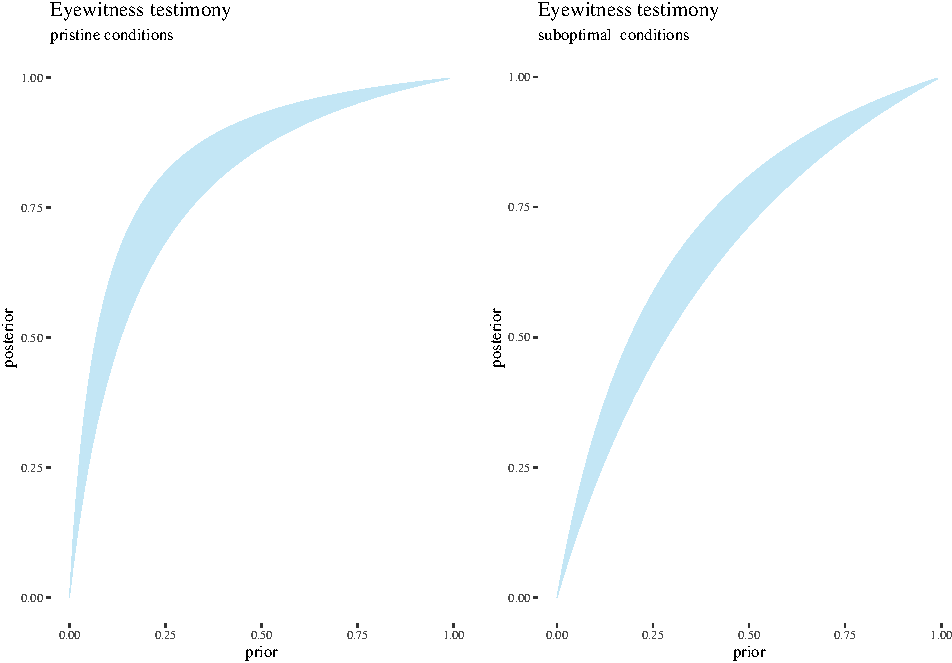
\includegraphics[width=1\linewidth]{lr-chapter4_files/figure-latex/eyewitness2b-1} \end{center}
\caption{Impact of an eyewitnss identification on the prior probability of the presence hypothesis under pristine and non-pristine conditions.}
\label{fig:eyewitness3b}
\end{figure}

\vspace{1mm}
\footnotesize

\normalsize

The examples could continue, but the general point is this. A
case-specific assessment of the risks of a false eyewitness
identification can be carried out by taking into account estimator and
system variables, as well as other relevant factors such as eyewitness
confidence. Ideally, properly formatted data about all the factors we
discussed could be used to develop a multivariate model. This model
would allow an assessment of the risks of error under a variety of
relatively well-specified circumstances. We are far from reaching this
state of maturity, but even with the current research, an expert who is
aware of the literature we have cited and of the specific circumstances
of the case could assess the risks of a false identification
quantitatively. An untrained jury member unaided by numerical
data---even after viewing cross-examination---is unlikely to arrive at a
better assessment of the risks of error involved.

We emphasize that the approach we are advocating here is continuous with
the practice of cross-examination. Questions that are routine during
cross-examination about time of day, distance, stress level, lighting
conditions etc.~elicit information about estimator variables as well as
system variables. Empirical research will help to determine how much
poor visibility, long distance, heightened stress, etc.~increase the
risk of a false identification. As noted before, the reason why
cross-examination is ineffective at detecting errors might well be that
it does not rely on data about the magnitude of the risks of error under
various circumstances. So, by combing numerical information in the
likelihood ratio, cross-examination can better serve its
purpose.\footnote{A word of caution is necessary, however. The mechanics
  of cross-examination is quite complex. While in general it is meant to
  elicit further information that should guide the evaluation of the
  evidence, there are a few different ways the situation might develop,
  and several argumentative moves that can be made in such a context. On
  one hand, the additional information obtained can \textit{rebutt} the
  eyewitness evidence, if it supports a hypothesis incompatible with the
  original one, as might happen when the eyewitness makes a statement
  contradicting something they have said previously. On the other, the
  new information might \textit{udercut} the eyewitness testimony if it
  leads to the re-evaluation of the witness's reliability without
  leading to a new hypothesis, as might happen when the eyewitness
  provides new evidence about the lightning conditions. This complexity
  cannot be satisfactorily modeled by using likelihood ratios only. It
  requires a more sophisticated formalism, Bayesian networks (Di Bello,
  2021). We will examine the mechanics of cross-examination in greater
  detail in another chapter.}\todo{refer to other chpater}

We conclude this section by addressing the question whether an
eyewitness identification is stronger or weaker evidence than a DNA
match. This is not only a question that is often a source of confusion,
but also a good opportunity to illustrate the applications of what we
have learned about match evidence (previous section) as well as
eyewitness testimony (this section).

So suppose the eyewitness evidence in a case is exculpatory but there is
also an incriminating DNA match. Which should prevail? It is tempting to
take a clear-cut position. For example, one could reason that DNA is
more reliable and thus should trump eyewitness evidence. Interestingly,
an appellate court in New York took a similar stance in People v. Rush,
165 Misc. 2d 821 (N.Y.~Sup.~Ct.~1995) . A rape victim identified the
defendant from a photograph a few weeks after the event. She also
identified the defendant in a line-up two weeks later. At trial,
however, she identified a spectator as her assailant, not the defendant.
So, the eyewitness evidence was mixed but ultimately exculpatory. On the
other hand, the defendant was seen in the vicinity of the crime scene
three days prior. A DNA expert testified to a positive match between the
crime scene genetic material and the defendant. The expert also
testified that the random match probability was 1 in 500 million.
Confronted with the question whether to believe the exculpatory
eyewitness testimony or the incriminating DNA match, the court wrote:

\begin{quote}
There can be little doubt, however, that the perils of eyewitness identification testimony far exceed those presented by DNA expert testimony ... This court is, therefore, satisfied that the testimony of even one DNA expert that there is a genetic match between the semen recovered from the victim of a rape and the blood of the defendant, a total stranger, and the statistical probability that anyone else was the source of that semen are 1 in 500 million is legally sufficient to support a guilty verdict.
\end{quote}

\noindent

We think such blanketed statements are unwarranted. The court framed the
question as one of whether a DNA match \textit{alone} can sustain a
conviction. It gave no weight to the exculpatory testimony. But, even
under this assumption, a random match probability of 1 over 500 million
corresponds to a likelihood ratio of 20 (if the false positive error
probability is .05) and 99 (if the false positive error probability is
.01).\footnote{We applied formula (\ref{eq:LRfp4b}), assuming a zero
  false negative probability FNP.} Are these numbers enough to convict?
Assume the DNA match speaks directly to the hypothesis of guilt, a
generous assumption in favor of the prosecution. By Bayes' theorem, if
the prior probability of the the guilt hypothesis is about .01, the
posterior guilt probability would be .5 (if the false positive
probability is .01) and .16 (if the false positive probability reaches
.05). These low numbers do not even take into account the exculpatory
testimony. Say the exculpatory testimony is assigned a likelihood ratio
of .5. This would bring the posterior guilt probability to .33 and .09
respectively, a far cry from what is needed to convict an
individual.\footnote{We multiplied the DNA match likelihood ratio by the
  exculpatory testimony likelihood ratio and then computed the posterior
  probability with Bayes' theorem. We examine how to combine different
  lines of evidence together in another chapter.}
\todo{refere to other chapter} \raf{M: Check calculations}

These numbers are merely illustrative, but they convey an important
lesson. The random match probability was fairly low, but to exclusively
rely on it was a mistake. As the previous section has shown, the false
positive probability can have a significant, negative impact on the
value of an incriminating match. In addition, it is true that eyewitness
testimony is fraught with problems. Its value might be low, especially
if the identification was not conducted under pristine conditions. But
without further details about estimator or system variables, it is hasty
to make sweeping statements that any eyewitness testimony is worthless.
This cautionary remark applies even more so to \textit{exculpatory}
testimony. The court reasoned that since the balance of the evidence
tipped markedly against the accused---because (incriminating) DNA
evidence outweighs (exculpatory) eyewitness evidence---this was enough
to convict. This is not quite right, however. Even if it has low value,
exculpatory eyewitness testimony can in principle weaken an
incriminating DNA match and create a reasonable doubt.\footnote{A more
  detailed discussion of standards of proof can be founding in Chapter
  XXX} The value of eyewitness testimony should neither be exaggerated
nor underestimated. As suggested in this section, a balanced assessment
can be achieved by incorporating---as part of the likelihood
ratio---numerical data about the risks of error under different
circumstances. \todo{ref to other chapter}

\hypertarget{hypothesis-choice}{%
\section{\texorpdfstring{Hypothesis choice
\label{sec:hchoice}}{Hypothesis choice }}\label{hypothesis-choice}}

The argument so far has shown that the likelihood ratio is a fruitful
conceptual framework for assessing the strength of the evidence, whether
it is a genetic match or eyewitness testimony. However, its deployment
is not devoid of challenges, and we move to a discussion of how they
arise. One major challenge is the choice of the hypotheses \(H\) and
\(H'\) that should be compared in the likelihood ratio. Generally
speaking, they should ``compete'' with one another---say, in a criminal
trial, \(H\) is put forward by the prosecution and \(H'\) by the
defense. But the two hypotheses need not be one the negation of the
other, and thus there is leeway in their selection. This leeway makes
the likelihood ratio quite versatile, but can also generate confusions
and misunderstandings in its interpretation.

The first confusion stems from using \textit{ad hoc} hypotheses. Suppose
the prosecutor argue that the suspect is the source of the traces found
at the crime scene. This claim is well supported by laboratory analyses
showing that the defendant genetically matches the traces. The defense,
however, responds by putting forward the following \textit{ad hoc}
hypothesis: `The crime stain was left by an unknown individual who
happened to have the same genotype as the defendant'. Since the
probability of the DNA match given either hypothesis is one, the
likelihood ratio equals one (Evett, Jackson, \& Lambert, 2000). The
problem generalizes. For any item of evidence and any hypothesis \(H\),
there is an \textit{ad hoc} competing hypothesis \(H^*\) that explains
the evidence just as well as \(H\) does, so
\(\nicefrac{\pr{E \vert H}}{\pr{E \vert H^*}}=1\) (Mayo, 2018). If no
further constraints are placed on the choice of the competing
hypotheses---it would seem---no evidence could ever incriminate anyone.

The confusion here consists in thinking that, since the likelihood
equals one, the evidence must be worthless. But this is a mistake. To be
sure, a genetic match cannot discriminate between hypothesis \(H\) (the
crime stain came from the defendant) and \(H^*\) (the crime stain came
from someone else who has the same genetic profile as the defendant).
They are both equally well-supported by the match. This is just a fact
about the world and a fact about how evidence works. The likelihood
ratio correctly tracks this fact. But since the likelihood ratio is
relative to a pair of hypotheses, the resulting assessment of the value
of the evidence is also relative. Even if the match has no evidential
value relative to \(H\) and \(H^*\), it may have---and most likely does
have---value relative to other hypotheses. It is a mistake to think that
a single likelihood ratio must be associated with a piece of evidence.
There are instead multiple likelihood ratios, each relative to a pair of
competing hypotheses.

A second confusion stems from failing to clearly articulate the
competing hypotheses, which then makes the assessment of the value of
the evidence meaningless. A good illustration of this point is the case
R.~v.~George (2007 EWCA Crim 2722). Barry George was accused of
murdering TV celebrity Jill Dando. The key piece of incriminating
evidence in the case was:

\begin{center}
\begin{tabular}{lp{12cm}} 
    $\textsf{residue}$ &  
    A single particle of firearm  residue was found one year later in George's coat pocket and matched the residue from the crime scene. 
\end{tabular}
\end{center}

\noindent  The defense argued that, since it was only one particle,
there must have been contamination. The expert for the prosecution,
however, testified that it was not unusual that a single particle would
be found on the person who fired the gun. George was convicted, and his
first appeal was unsuccessful.

After the first appeal, Dr.~Evett from the Forensic Science Service in
the United Kingdom worried that the evidence had not been properly
assessed at trial. The jurors were presented with the conditional
probability \(\pr{\textsf{residue}\vert H_d}\) of finding the firearm
residue in George's coat given the defense hypothesis \(H_d\) (say, that
George \textit{did not} fire the gun). This probability was estimated to
be quite low, indicating that the evidence spoke against the defense's
hypothesis. But the jurors were not presented with the conditional
probability \(\pr{\textsf{residue}\vert H_p}\) of finding the same
evidence given the prosecutor's hypothesis \(H_p\) (say, that George
\textit{did} fire the gun). An expert witness, Mr.~Keeley, was asked to
provide both conditional probabilities and estimated them to be
\(\nicefrac{1}{100}\), which indicated that the firearm residue had no
probative value. After new guidelines for reporting low level of firearm
residue were published in 2006, the Forensic Science Service re-assessed
the evidence and concluded that it was irrelevant. George appealed again
in 2007, and relying on Keely's estimates, won the appeal.

At first, this case seems a good illustration of how likelihood ratios
help to correctly asses the value of the evidence presented at trial.
But what were the hypotheses that the expert compared? A study of the
trial transcript shows that Keeley's choice of hypotheses was not
transparent and the likelihood ratio based on them was therefore hard to
interpret (Fenton, Berger, Lagnado, Neil, \& Hsu, 2014). On one
occasion, Keeley took the prosecutor's hypothesis to be `The particle
found in George's pocket came from the gun that killed Dando' and the
defense hypothesis to be `The particle on George's pocket was inserted
by contamination.' The problem is that the evidence is a logical
consequence of either of them, so the conditional probability of the
evidence given each hypothesis is one. The most charitable reading of
the trial transcript suggests that the expert had in mind the hypotheses
`George was the man who shot Dando' and `The integrity of George's coat
was corrupted.' But Keeley was never clear that he compared these two
hypotheses. Thus, the meaning of the likelihood ratio he provided
remains elusive (see Fenton, Berger, Lagnado, Neil, \& Hsu, 2014 for
further details).

The confusion in the George case stems from the lack of a clear
statement of the hypotheses. This lack of clarity can lead one to think
that, since the likelihood ratio equals one (for a pair of not
well-specified competing hypotheses), the evidence must prove nothing.
To avoid this slippage, experts should perhaps only pick hypotheses that
are exclusive (they cannot be both true) and exhaustive (they cannot be
both false). In this way, the parties would not be able to pick
\textit{ad hoc} hypotheses and skew the assessment of the evidence in
their own favor. Further, exclusive and exhaustive hypotheses would have
likely forced the expert in the George case to be more precise.

But requiring that the hypotheses be always exclusive and exhaustive is
not without complications either. Conceptually, it is a good idea to
compare a hypothesis with its negation. Practically, this might not be
viable, as often there are multiple different ways a hypothesis can turn
out to be false. For consider an expert who decides to formulate the
defense hypothesis by negating the prosecution hypothesis, say, `the
defendant did \textit{not} hit the victim in the head.' This choice for
the defense hypothesis can be unhelpful in assessing the evidence,
because the required probabilities are hard to estimate. What is the
probability that the suspect would carry such and such blood stain if he
did not hit the victim in the head? This depends on whether he was
present at the scene, what he was doing at the time and many other
circumstances. As Evett, Jackson, \& Lambert (2000) point out, in many
real life cases, the choice of a particular hypothesis to be used by the
expert in the evaluation of the evidence will depend on contextual
factors.\footnote{Another practical difficulty is that comparing
  exclusive and exhaustive hypotheses can be unhelpful for jurors or
  judges. In a paternity case, for example, the expert should not
  compare the hypotheses `The accused is the father of the child' and
  its negation, but rather, `The accused is the father of the child' and
  `The father of the child is a man unrelated to the putative father'
  (Biedermann, Hicks, Taroni, Champod, \& Aitken, 2014). The choice of
  the latter pair of competing hypotheses is preferable. Even though the
  relatives of the accused are potential fathers, considering such a
  far-fetched possibility would make the assessment of the evidence more
  difficult than needed.}

A third confusion stems from the fact that pairs of roughly similar
hypotheses---which provide descriptions of the events at different
levels of granularity---may be associated with different likelihood
ratios for the same evidence (Fenton, Berger, Lagnado, Neil, \& Hsu,
2014). This variability makes the likelihood ratio a seemingly arbitrary
and easily manipulable measure of evidential value. An intriguing
example of this phenomenon is a variation on the two-stein problem,
originally formulated by Evett (1987). Suppose a crime was committed by
two people, who left two stains at the crime scene: one on a pillow and
another on a sheet. John Smith, who was arrested for a different reason,
genetically matches the DNA on the pillow, but not the one on the
sheet.\footnote{In the original formulation, two stains from two
  different sources were left at the crime scene, and the suspect's
  blood matches one of them. Let one hypothesis be that the suspect was
  one of the two men who committed the crime and the other hypothesis
  the negation of the first. Evett (1987) shows that the likelihood
  ratio of the match relative to these two hypotheses is
  \(\nicefrac{1}{2q_1}\) where \(q_1\) is the estimated frequency of the
  characteristics of the first stain. The likelihood ratio does not
  depend on the frequency associated with the second stain. In general,
  if there are \(n\) bloodstains of different phenotypes, the likelihood
  ratio is \(\nicefrac{1}{nq_1}\). So the likelihood ratio depends on
  the number of stains but not on the frequency of the other
  characteristics.} What likelihood ratio should we assign to the DNA
match in question? Meester \& Sjerps (2004) argue that there are three
plausible pairs of hypotheses associated with numerically different
likelihood ratios (see their paper for the derivations). The three
options are listed below, where 1 in \(R\) is the random match
probability of Smith's genetic profile and \(\delta\) the prior
probability that Smith was one of the crime scene donors. \vspace{2mm}

\begin{center}
    \footnotesize
    \begin{tabular}{@{}p{5cm}p{5cm}l@{}}
        \toprule
        $H_p$ & $H_d$  & LR \\ \midrule
        Smith was one of the crime scene donors.   &  Smith was \textit{not} one of the crime scene donors. & $\nicefrac{R}{2}$   \\
        Smith was the pillow stain donor.     & Smith was not one of the crime scene donors.& $R$\\
        Smith was the pillow stain donor. & Smith was not the pillow stain donor. &  $\nicefrac{R(2-\delta)}{2(1-\delta)}$
        \\ \bottomrule
    \end{tabular}
\end{center}
\normalsize
\vspace{2mm}

\noindent The first pair of hypotheses is the most general, encompassing
any trace at the crime scene. The third pair is the most specific,
focusing on just the trace on the pillow . The second pair lies in
between the other two. There is significant variability across the three
likelihood ratios. The first is half the second and third likelihood
ratios (if \(\delta\) is close to zero). In a trial, we could imagine
prosecution and defense disagreeing about the right selection of
hypotheses to compare. To their advantage, the prosecution might insist
that the right comparison is given by the second or third pair, while
the defense might insist that the right comparison is given by the first
pair.

A closer scrutiny of the matter, however, reveals that the difference
across likelihood ratios is not as troubling as it might seem. It would
be surprising that the likelihood ratio for the same piece of evidence
would remain the same when it is applied across hypotheses that make
different commitments about what happened. So, once again, the
likelihood ratio behaves as it should. It finely discriminates between
the granularity of different hypotheses.\footnote{Interestingly, even
  though the likelihood ratios are numerically different, the posterior
  odds for the three pair of hypotheses are the same. To see why, note
  that the prior odds of the three \(H_p\)'s in the table should be
  written in terms of \(\delta\). Following Meester \& Sjerps (2004),
  the prior odds of the first hypothesis in the table are
  \(\nicefrac{\delta}{1-\delta}\). The prior odds of the second
  hypothesis are \(\nicefrac{(\delta/2)}{(1-\delta)}\). The prior odds
  of the third hypothesis are \(\nicefrac{(\delta/2)}{(1-(\delta/2))}\).
  In each case, the posterior odds --- the result of multiplying the
  prior odds by the likelihood ratio --- are the same:
  \(R\times \nicefrac{\delta}{2(1-\delta)}\). The reason for this is
  that the hypotheses are equivalent conditional on the evidence. Smith
  was one of the crime scene donors just in case he was the pillow stain
  donor, because he is excluded as the stain sheet donor. Smith was not
  one of the crime scene donors just in case he was not the pillow stain
  donor, because he is excluded as the sheet stain donor. Dawid (2004)
  cautions that the equivalence of hypotheses, conditional on the
  evidence, does not imply that they can all be presented in court.
  Meester \& Sjerps (2004) recommend that the likelihood ratio should be
  accompanied by a tabular account of how a choice of prior odds (or
  prior probabilities) will impact the posterior odds, for a sensible
  range of priors.}

The moral is this. The likelihood ratio is perfectly fine in its place,
but its limits should be kept in mind. We should not overlook that it is
relative to a pair of hypotheses and thus its assessment of the evidence
is also relative. So we are dealing with a two-step process here: first,
select a pair of hypotheses of interest; and second, assess whether the
evidence makes a distinction between the two and to what extent. The
likelihood ratio is useful for the second step, not the first. It
provides no guidance in choosing the hypotheses. It is a tool to assess
the value of the evidence \textit{once} the hypotheses are chosen. The
two steps must be spelled out clearly and kept separate. If they are
not, confusions and misinterpretations of the evidence will occur. As
noted at the start of this chapter, we are after a \textit{local}
measure of evidential value (strength, support), one that is
circumscribed to a certain hypothesis or pair of hypotheses. The
likelihood ratio serves this purpose well, but does nothing more than
that. We elaborate on this point further as we discuss the notion of
legal relevance in the next and final section.

\hypertarget{relevance-and-the-small-town-murder-scenario}{%
\section{\texorpdfstring{Relevance and the small-town murder scenario
\label{sec:relevance}}{Relevance and the small-town murder scenario }}\label{relevance-and-the-small-town-murder-scenario}}

The Federal Rules of Evidence define relevant evidence as one that has
`any tendency to make the existence of any fact that is of consequence
to the determination of the action more probable or less probable than
it would be without the evidence' (rule 401). As before, we are dealing
with a two-step process here: first, select a `fact that is of
consequence to the determination of the action,' sometimes called a
material fact or hypothesis; and second, assess whether the evidence
changes the probability of the material fact or hypothesis. More
succinctly, two conditions must be met: (1) materiality and (2)
probative value. An item of evidence is relevant if it has probative
value for a hypothesis that is material (`of consequence to the
determination of the action'). The likelihood ratio is helpful for
assessing probative value, and in fact, it allows for a more
fine-grained assessment because it formalizes \textit{degrees} of
probative value (or strength, support). We have illustrated how this can
be done in the case of match evidence and eyewitness testimony. But the
likelihood ratio does not directly address the question of materiality
and therefore cannot provide a full account of relevance.

Consider now probative value more closely. The Rules define it in
probabilistic language, an occurrence that has not gone unnoticed (CGG
Aitken, Roberts, \& Jackson, 2010; Colin Aitken \& Taroni, 2004;
Lempert, 1977; Lyon \& Koehler, 1996; Sullivan, 2019). Specifically, the
Rules invoke the idea of a probability change, but do not mention the
likelihood ratio. The two are related, however. A piece of evidence
changes the probability of hypothesis \(H\) \textit{if and only if} the
likelihood ratio \(\nicefrac{\pr{E \vert H}}{\pr{E\vert \neg H}}\) is
different from one. But note that the comparison here holds between
\(H\) and its negation, not just between any two competing hypotheses
\(H\) and \(H'\). When the comparison is between hypotheses that are not
one the negation of the other, likelihood ratio and probability change
come apart. A piece of evidence may change the probability of a
hypothesis---so that \(\pr{H \vert E}\neq \pr{H}\)---even though the
likelihood ratio \(\nicefrac{pr{E \vert H}}{\pr{E\vert H'}}\) equals
one. How can that be?

Suppose Fred and Bill attempted to rob a man. The victim resisted, was
struck on the head and died. Say \(H_p\) stand for `Fred struck the
fatal blow' and \(H_d\) stand for `Bill struck the fatal blow.' The
hypotheses are not exhaustive. A missing hypothesis is `The man did not
die from the blow.' Suppose \(E\) is the information that the victim had
a heart attack six months earlier. The likelihood ratio
\(\nicefrac{\pr{E \vert H_p}}{\pr{E \vert H_d}}\) equals one since
\(\pr{E\vert H_p}=\pr{E\vert H_d}\). Yet \(E\) reduces the probability
of both \(H_p\) and \(H_d\). This might be confusing, but there is no
inconsistency here. If what is material in the case is only whether
either Bill or Fred did it, evidence about a heart attack would be
irrelevant. The likelihood ratio correctly tracks this fact. On the
other hand, if what is material is whether the victim died by natural or
human causes, evidence about a heart attack would be relevant. Again, it
is paramount not to confuse questions of materiality and questions of
probative value.

The distinction between materiality and probative value also helps to
deflect the force of a number of counterexamples against the likelihood
ratio that we find in the literature. The vignette below was formulated
by Ronald Allen and appears in the multi-authored discussion in (Park et
al., 2010):

\begin{quote}
    \textbf{Small Town Murder.} A person accused of murder in a small town was seen driving to the small town at a time prior to the murder. The prosecution's theory is that he was driving there to commit the murder. The defense theory is an alibi: he was driving to the town because his mother lives there to visit her. The probability of this evidence if he is guilty equals that if he is innocent, and thus the likelihood ratio is 1 \dots , and under what is suggested as the "Bayesian" analysis, it is therefore irrelevant. 
    Yet, every judge in every trial courtroom ... would say it is relevant.  And so we have a puzzle.  
    \end{quote}

\noindent  Counterexamples of this sort abound.\footnote{Here is another
  scenario: Suppose a prisoner and two guards had an altercation because
  the prisoner refused to return a food tray. The prisoner had not
  received a package sent to him by his family and kept the tray in
  protest. According to the defense, the prisoner was attacked by the
  guards, but according to the prosecution, he attacked the guards. The
  information about the package sent to the prisoner and the withholding
  of the tray fails to favor either version of the facts, yet it is
  relevant evidence (Pardo, 2013).} The puzzle is that the evidence is
intuitively relevant and yet the likelihood ratio would seem to tell
otherwise. There are a few things to say in response. First, as noted
already, the likelihood ratio provides an account of probative value
(strength, support), not relevance (which includes both materiality and
probative value). Further, probative value is relative to a specific
pair of hypotheses. The likelihood ratio may change depending on the
selection of hypotheses.

Rule 401 makes clear that relevant evidence should have `any tendency to
make the existence of \emph{any fact that is of consequence} {[}emphasis
ours{]} to the determination of the action more probable or less
probable.' Just because the likelihood ratio equals one for a specific
selection of \(H\) and \(H'\), it does not follow that it equals one for
\textit{any} selection of \(H\) and \(H'\) which are of consequence to
the determination of what happened. For example, the likelihood ratio of
the evidence `suspect was seen driving to town' relative to the pair of
hypotheses `suspect was in town' \textit{versus} `suspect was not in
town' would be different from one. Whether the suspect was in town at
all is presumably of consequence for determining what happened. So the
fact that he was seen driving is helpful information for establishing
whether or not he was in town, and the likelihood ratio can model this
fact.

This discussion makes clear that relevance is a
\textit{global, holistic} notion. Legal cases often have a very complex
structure. They consist of several pieces of evidence as well as several
factual hypotheses to be assessed in light of the evidence. Some may be
all-encompassing, such as the ultimate prosecutor's hypothesis `The
defendant committed insider trading.' Other hypotheses may be more
circumscribed, such as `The defendant visited the victim on Sunday.' An
item of evidence is relevant so long as it can affect the probability of
\textit{any} material hypothesis, in one way or another.\footnote{A
  complication is that the choice of hypotheses needed to determine
  relevance might depend on other items of evidence, and so it might be
  difficult to determine relevance until one has heard all the evidence.
  This fact---Ronald Allen and Samuel Gross argue in (Park et al.,
  2010)---makes the probabilistic account of relevance impractical. But,
  in response, David Kaye points out that deciding whether a reasonable
  juror would find evidence \(E\) helpful requires only looking at what
  hypotheses or stories the juror would reasonably consider. Since the
  juror will rely on several clues about which stories are reasonable,
  this task is computationally easier than going over all possible
  combinations of hypotheses (Park et al., 2010).} Evidence is relevant
so long as it has a probabilistic impact on a sub-hypothesis involved in
the case, even without having a recognizable probabilistic impact on the
prosecutor's or defense's ultimate hypotheses. A local assessment of the
value of the evidence using the likelihood ratio can help to make
decisions about relevance. But in order to model the relationships
between hypotheses formulated at different levels of complexity, we need
to move past the likelihood ratio. As we shall see in later chapters,
Bayesian networks can make better sense of this holistic perspective (de
Zoete, Fenton, Noguchi, \& Lagnado, 2019).

\hypertarget{conclusion}{%
\section{Conclusion}\label{conclusion}}

We discussed the likelihood ratio as a measure of evidential value
(strength, support). We argued that it is a better fit in the legal
settings than the Bayes factor. It is not heavily dependent on prior
probabilities, it is flexible and is not liable to the problem of
irrelevant conjuncts. We illustrated how the likelihood ratio can be
deployed for evaluating match evidence and eyewitness testimony. We
emphasized how it provides a conceptual framework that can be filled in
with numerical data about the risks of error, false positive and false
negative probabilities. This approach promises to strengthen the role of
cross-examination as a tool for weeding out bad evidence.

But despite its promise, the likelihood ratio has limits. It is relative
to a pair of (often rather circumscribed) hypotheses and its meaning
should not be severed from them. Strictly speaking, there is no single
likelihood ratio that corresponds to a single piece of evidence.
Multiple hypotheses can be at issue in a legal case and the same piece
of evidence can speak to them to different degrees. There is nothing
surprising about that. Circumscribed sub-hypotheses are part of larger,
more complex hypotheses, and finally, they all converge into the
ultimate hypothesis. To model these complex relationships, however, a
more elaborate theoretical framework is needed, Bayesian networks, our
topic in several chapters to follow.

\appendix

\addcontentsline{toc}{section}{Appendices}

\section{ Confirmation measures \label{sec:confirmation}}

Our terminology in this chapter included expressions such as `strength
of evidence,' `value of evidence' or `evidential support.' An expression
often used in the philosophical literature is `confirmation.' How is
confirmation related to the discussion in this chapter? Bayesian
confirmation theory is sub-field of philosophy of science and
epistemology. It aims to provide a probabilistic account of what it
means for evidence to confirm a scientific theory. This naturally bears
similarities with the question of what it means for evidence to support
a hypothesis put forward of the prosecution or the defense in a trial.
We will briefly summarize some of the theories of Bayesian confirmation
out there and then compare confirmation to evidential strength (or
value, support).

Confirmation can be understood as function of agent's degrees of
belief---a measure of an agent's \textit{firmness} of belief. On this
account, the degree of confirmation that a piece of evidence \(E\)
provides in favor of scientific theory \(T\) is defined as the posterior
probability \(\pr{T \vert E}\). This account can be defended by invoking
three plausible requirements that any measure of confirmation should
satisfy.

The first requirement is that the degree of confirmation is a continuous
function of \(\pr{T}\) and \(\pr{E\vert T}\) which is non-decreasing in
the first argument and non-increasing in the second argument. That is,
increasing the prior, should not lower the confirmation level, and
increasing the likelihood should not increase the confirmation level
(Sprenger \& Hartmann, 2019) is . Call this condition the
\emph{prior-posterior dependence}.\footnote{Some formulations (Crupi,
  2015) are a bit more general and include background knowledge \(K\).
  In that setting, the corresponding requirement is called
  \emph{Formality} and takes the confirmation to be a function of
  \(\pr{H \et E \vert K}, \pr{H\vert K}\) and \(\pr{E\vert K}\). For the
  sake of simplicity, we will suppress the reference to \(K\), unless
  required by the context.} A corollary of the
prior-posterior-dependence is that confirmation of \(T\) by \(E\),
\(c(T,E)\) should track the posterior order-wise, that is
\(c(T,E)>c(T,E')\) just in case \(\pr{T\vert E} > \pr{T\vert E'}\). A
second requirement is that there should be a neutral point \(n\) such
that \(E\) confirms (disconfirms) \(T\) just in case \(c(T,E)>n\)
(\(c(T,E)<n\)) and is neutral exactly at \(n\). Call this the
\emph{qualitative-quantitative bridge}. Finally, a third requirement is
\emph{local equivalence}. Theories that are logically equivalent given
the evidence should receive equal confirmation from this evidence.

Interestingly, all confirmation measures which satisfy prior-posterior
dependence, qualitative-quantitative bridge, and local equivalence are
strictly increasing functions of \(\pr{H \vert E}\). Such measures are
said to explicate confirmation as \emph{firmness of belief}. Moreover,
all functions satisfying these three conditions are ordinally
equivalent.\footnote{Measure $c$ is ordinally equivalent to measure $c'$ just in case always $c(E , T) \gtreqqless c(E', T')$ iff $c'(E , T) \gtreqqless c'(E' , T')$.}

But the concept of confirmation cannot be fully captured by posterior
probabilities. Even if the posterior \(T\) is low, one might still think
that a given experiment speaks strongly in favor of \(T\). And
converserly, \(E\) can lower the posterior of \(T\) while still leading
the posterior to be sufficiently high for the firmness confirmation
measure to be above the neutrality threshold. Another feature of
confirmation as firmness is that if, in this sense, \(T\) confirms
\(H\), then for any \(H'\) that is excluded by \(H\), \(T\) disconfirms
\(H'\). But now think of the small town murder scenario we already
discussed: the fact that the suspect was seen in town seems to support
both the prosecution hypothesis that he committed the murder, and the
defense hypothesis, that he was in town to visit his mother.
Confirmation as firmness cannot capture such intuitions, as relevance
cannot be captured as a function of the posterior alone.

For such reasons, following the second edition of (Carnap, 1962), it is
customary to distinguish another notion in the vicinity: confirmation as
\textit{increase in firmness} of belief. If we replace local equivalence
with tautological equivalence \(c(T, \top) = c(T', \top)\), where
\(\top\) is a logical tautology---the idea being that hypotheses are
equally supported by empty evidence---we end up with another class of
confirmation measures, those meant to capture
\emph{probabilistic relevance}. On this approach, \(E\) confirms
(disconfirms) \(T\) just in case \(\pr{H \vert E} > \pr{H}\)
(\(\pr{H \vert E} < \pr{H}\)).

Here is a list of the most prominent confirmation measures on offer
(Sprenger \& Hartmann, 2019), normalized so that they all have neutral
points at 0:

\begin{align}
\tag{Difference}  D(T,E) & = \pr{T\vert E} - \pr{T}\\
\tag{Log-ratio}  Lr(T,E) &  = log\left(\frac{\pr{T\vert E}}{\pr{T}} \right) \\
\tag{Log-likelihood}   LL(T,E) & = log\left(\frac{\pr{E \vert T}}{\pr{E \vert \n T}} \right)\\
\tag{Kemeny-Oppenheim}  K(T,E) & = \frac{\pr{E\vert T} - \pr{E \vert \n T}}{\pr{E \vert T} + \pr{E \vert \n T}} \\
\tag{Generalized entailment}  Z(T,E) & = \begin{cases}
\frac{\pr{T\vert E} - \pr{T}}{1-\pr{T}} & \mbox{ if } \pr{T \vert E} \geq \pr{T}\\
\frac{\pr{T\vert E} - \pr{T}}{\pr{T}} & \mbox{ if } \pr{T \vert E} < \pr{T}
\end{cases} \\
\tag{Christensen-Joyce} S(T,E) & = \pr{T \vert E} - \pr{T \vert \n E} \\
\tag{Carnap}  C(T,E) & = \pr{E}(\pr{T\vert E} - \pr{T})\\
\tag{Rips} R(T\vert E) & = 1 - \frac{\pr{\n T\vert E}}{\pr{-T}}
\end{align}

\noindent The Log-likelihood, the Kemeny--Oppenheim measure and the
simple likelihood ratio (not in the list above) are ordinally equivalent
(and no other pair on the list is). Log-likelihood makes calculations of
joint support additive, and the the Kemeny--Oppenheim measure has the
nice feature of ranging from \(-1\) to \(1\) and having 0 as a neutral
point. If one accepts the likelihood ratio, these two can be used on
some occasions when these additional features are needed

The choice of one's preferred confirmation measure is aided by the
following facts:

\begin{itemize}
\item
  Consider the requirement that \(E\) always confirms the disjunction of
  excluding hypotheses more than one of them just in case it also
  confirms the other one (\emph{disjunction of alternative hypotheses}).
  \raf{M: This is not clear. What does that mean?}. This requirement is
  satisfied only by a confirmation measure that is a strictly increasing
  function of the difference measure. Whether this is an intuitive
  requirement in the legal setting is unclear.
\item
  The requirement that confirmation track likelihood, that is,
  \(c(T,E) > c(T,E')\) just in case \(\pr{E\vert T} > \pr{E'\vert T}\)
  (\emph{Law of likelihood}) is met only if the measure is a strictly
  increasing function of the Bayes factor. In legal applications, the
  law of likelihood is suspicious, as our example with rocking child
  abuse victims discussed on page \ref{text:rock} indicates.
\item
  The requirement that confirmation be \emph{contrapositive}
  (\(c(T,E) = c(\n E, \n T))\) and \emph{commutative}
  (\(c(H,E) = c(E,H)\)) is met only by relative distance measures, that
  is, strictly increasing functions of the generalized entailment
  measure.
\item
  Consider the requirement that if \(E\) and \(E'\) are conditionally
  independent given \(T\) and \(\neg T\), then \(c(T,E)\) should be
  identical with \(c(T,E\vert E')\) (the confirmation obtained when
  \(E'\) is added to the background knowledge). Call this called
  \emph{modularity}. This requirement holds only if a confirmation
  measure is a strictly increasing function of the likelihood ratio.
\item
  If one requires strict
  additivity---\(c(H, E\et E') = c(H, E) + c(H, E'\vert E)\)---the only
  measure that satisfies the disjunction of alternative hypotheses is
  the difference measure; the only measure that satisfies the law of
  likelihood is the log-ratio measure; and the only one that satisfies
  modularity is the log-likelihood measure.
\end{itemize}

So we face a seemingly radical plurality of confirmation measures. These
measures, however, can be unified by a normalizing procedure described
in (Crupi, Tentori, \& Gonzalez, 2007). Leaving out the details, these
different measures are equivalent to the following:

\begin{align*}
Z_{\alpha}  & =  \left\{ \begin{array}{lr} 
Z(h, e)^{\alpha} & \mbox{ if } \pr{T\vert E} \geq \pr{T}\\
- |Z(h, e)|^{\alpha} &\mbox { otherwise.}\\
\end{array} \right.
\end{align*}

\noindent \(Z_{\alpha}\) is an S-shaped function where the parameters
\(\alpha\) describes the curvature. So \(Z_{\alpha}\) defines a family
of measures, call them Z-measures. One strong reason to favor them is
that they generalizes logical entailment. Take any \(k > 0\) and say
\(v(E,T) =k\) iff \(E\models T\), \(v(E,T) = -k\) iff \(E \models \n T\)
and \(v(E,T)=0\) otherwise. Call \emph{logical closure} the requirement
that if \(v(E,T) > v(E', T')\), then \(c(E, T) > c(E' , T' )\). Logical
closure is satisfied only by the generalized entailment measure and the
likelihood ratio (along with the ordinally equivalent measures, the
Log-likelihood and Kemeny-Oppenheim measure). The other measures fail to
satisfy this requirement.

Besides failure of logical closure, there are further reasons to reject
the other measures. First, Carnap's and Christensen-Joyce's measure fail
to meet the requirement of prior-posterior dependence. Second, Carnap's
measure and Log-ratio have the counterintuitive consequence that
\(C(T,E)= C(E,T)\) (call this \emph{symmetry}). Third, the difference
measure, generalized entailment, the Log-ratio, Carnap's and Rips's
measures depend on the prior of \(T\). So the only mesure that stand are
the likelihood ratio (and the ordinarilly equivalent measures) and the
Z-measures. But the latter suffer from a problem identified by Branded
Fitelson (2021). Say \(E\) and \(E'\) are confirmationally independent
regarding \(H\) just in case both \(c(T, E \vert E' ) = c(T, E )\) and
\(c(T, E' \vert E ) = c(T, E')\) Say \(E\) and \(E'\) are conflicting
evidence regarding \(T\) iff \(\pr{T\vert E}> \pr{T}\) while
\(\pr{T\vert E'} < \pr{T}\). Branded Fitelson (2021) has proven that any
measure ordinally equivalent with \(Z\) excludes the fairly intuitive
possibility of the existence of confirmationally independent and yet
conflicting evidence.

Dependence on prior probabilities is particularly problematic in the
legal setting. On the other hand, in legal context, we would like (1)
the expert's assessment not to depend on the expert's prior convictions
about the hypothesis, and (2) the expert's statement to mean the same
for various agents involved in the fact-finding process, even if they
assign different priors to the hypothesis. For this reason, we hold that
dependence on priors in legal evidence evaluation is an undesirable
feature of a confirmation measure. This might be less pressing in the
scientific setting. Say a scientific community agrees on the status of a
given theory prior to an experiment. Then, after the experiment, it is a
legitimate question what impact the experiment has on the status of that
theory, and perhaps it makes sense that the prior status of that theory
plays a role in the theory's confirmation.

Table \ref{tab:confirmation} summarizes the reasons not to adopt a
certain measure of confirmation. The likelihood ratio emerges as the
clear winner. The Log likelihood and Kemeny-Oppenheim's measures are
ordinally equivalent to the likelihood ratio. The reason to not use them
in the legal setting is mostly a matter of convenience.
Kemeny-Oppenheim's is conceptually more complex than likelihood ratio,
and thinking in terms of logarithms is unnatural for ordinary
reaosoners.

\begin{table}
\centering\begingroup\fontsize{9}{11}\selectfont

\begin{tabular}{lp{10cm}}
\toprule
Measure & Reason not to use\\
\midrule
\cellcolor{gray!6}{(Difference)} & \cellcolor{gray!6}{dependence on priors, logical closure failure}\\
(Log-ratio) and (Bayes factor) & satisfies law of likelihood, symmetry, dependence on priors, failure to satisfy logical closure\\
\cellcolor{gray!6}{(Generalized entailment)} & \cellcolor{gray!6}{dependence on priors, independent conflicting evidence}\\
(Christensen-Joyce) & excluded by final probability incrementality with prior-posterior dependence\\
\cellcolor{gray!6}{(Carnap)} & \cellcolor{gray!6}{excluded by final probability incrementality with prior-posterior dependence, symmetry, logical closure failure}\\
(Rips) & dependence on priors, failure of logical closure\\
(Christensen-Joyce) & excluded by final probability incrementality with prior-posterior dependence\\
\cellcolor{gray!6}{(Kemeny-Oppenheim)} & \cellcolor{gray!6}{none of the above, but unnecessarily complex}\\
(Log likelihood) & none of the above, but logarithms are hard for humans\\
\cellcolor{gray!6}{(Likelihood ratio)} & \cellcolor{gray!6}{none of the above}\\
\bottomrule
\end{tabular}
\endgroup{}
\caption{Reasons not to use various confirmation measures in legal fact-finding applications.}
\label{tab:confirmation}
\end{table}

Finally, we should mention a general argument for preferring the
likelihood ratio. This argument was developed by Heckerman (1988).
Suppose you have background information \(b\), and consider a hypothesis
\(H\) when you obtain a piece of evidence \(E\). A belief update,
\(U(H, E, b)\), together with your prior stance about \(H\), should
determine your posterior belief in \(H\). If we denote conditional
belief in \(H\) given \(E\), without assuming it is probabilistic yet,
as \(H\vert E\), this means that there should be a function \(f\) such
that: \begin{align*}
H \vert E, b & = f(U(H,E,b), H \vert b)
\end{align*}

\noindent where, on this approach, \(H \vert E, b\) and \(U(H,E,b)\) and
\(H \vert b\) are all real numbers, and \(f\) is required to be
continuous in both arguments and monotonically increasing when the other
is held constant. Call this the \textit{update requirement}. Bayesian
updating is a particular case: the selection of \(H\) and \(b\), with a
joint distribution in the background, determines a function from
\(\pr{H \vert b}\) to \(\pr{H \vert E, b}\).

Further, assume the \textit{consistency property}: if the arguments are
logically equivalent, then belief update yields the same value:
\begin{align*}
[H_1 \Leftrightarrow H_2, E_1 \Leftrightarrow E_2] \Rightarrow U(H_1, E_1, b_1) = U(H_2, E_2, b_2)
\end{align*}

The next assumption has it that when you update on two items of
evidence, the order of updating shouldn't matter and the result should
be the same as updating on the joint evidence. The
\textit{combination property} requires that there is a function \(g\)
that is continuous in both arguments and monotonically increasing in
each argument when the other is held constant such that: \begin{align*}
U(H, E_1E_2,b) & =  g(U(H,E_1, b), U(H, E_2, E_1, b))
\end{align*} A general result in group theory by Aczel is that any
continuous monotonic function of two arguments that satisfies the
associativity relation must be additive in some transformed space. In
this particular case, the result entails that any update that satisfies
the update condition, and the consistency and combination properties is
the arithmetic difference of a posterior and prior belief up to an
arbitrary monotonic transformation, that is, that there are monotonic
functions \(h\) and \(i\) such that: \begin{align*}
h(U(H,E,b)) & = i(H\vert E, b) - i(H\vert b)
\end{align*} In the probabilistic context, where \(H\vert E\) is
\(\pr{H\vert E}\), the likelihood ratio satisifies the update
requirement and has the combination and consistency properties.
Accordingly, the transformation that makes it additive is the
logarithmic function.

Now, the \emph{independence correspondence property} has it that if
\(E_1\) and \(E_2\) are conditionally independent given \(H\) and given
\(\n H\), then \(U(H, E_2, E_1, b) = U(H, E_2, b)\). The key result is
that any probabilistic update satisfying the independence correspondence
must be a monotonic transformation of the likelihood ratio. This means
that there is a list of fairly intuitive general conditions on what an
update function should behave like which entails that it is just a
variant of the likelihood ratio.

\hypertarget{references}{%
\section*{References}\label{references}}
\addcontentsline{toc}{section}{References}

\hypertarget{refs}{}
\begin{CSLReferences}{1}{0}
\leavevmode\hypertarget{ref-aitken2010fundamentals}{}%
Aitken, CGG, Roberts, P., \& Jackson, G. (2010). Fundamentals of
probability and statistical evidence in criminal proceedings
({P}ractitioner {G}uide {N}o. 1), {G}uidance for judges, lawyers,
forensic scientists and expert witnesses. \emph{Royal Statistical
Society's Working Group on Statistics and the Law}.

\leavevmode\hypertarget{ref-aitken2004statistics}{}%
Aitken, Colin, \& Taroni, F. (2004). \emph{Statistics and the evaluation
of evidence for forensic scientists} (Vol. 16). Wiley Online Library.

\leavevmode\hypertarget{ref-aitken2008fundamentals}{}%
Aitken, Colin, \& Taroni, F. (2008). Fundamentals of statistical
evidence - a primer for legal professionals. \emph{The International
Journal of Evidence and Proof}, \emph{12}(3), 181--207. SAGE
Publications.

\leavevmode\hypertarget{ref-aitken2003probability}{}%
Aitken, Colin, Taroni, F., \& Thompson, W. (2003). How the probability
of a false positive affects the value of DNA evidence. \emph{Journal of
Forensic Science}, \emph{48}(1), 1--8. ASTM International.

\leavevmode\hypertarget{ref-behrman2001EyewitnessIdentificationActual}{}%
Behrman, B. W., \& Davey, S. L. (2001). Eyewitness identification in
actual criminal cases: {An} archival analysis. \emph{Law and Human
Behavior}, \emph{25}(5), 475--491.

\leavevmode\hypertarget{ref-bickel2012strength}{}%
Bickel, D. R. (2012). The strength of statistical evidence for composite
hypotheses: Inference to the best explanation. \emph{Statistica Sinica},
1147--1198. JSTOR.

\leavevmode\hypertarget{ref-biedermann2014UseLikelihoodRatio}{}%
Biedermann, A., Hicks, T., Taroni, F., Champod, C., \& Aitken, C.
(2014). On the use of the likelihood ratio for forensic evaluation:
{Response} to {Fenton} et al. \emph{Science \& Justice}, \emph{54}(4),
316--318.

\leavevmode\hypertarget{ref-buckleton2018forensic}{}%
Buckleton, J. S., Bright, J.-A., \& Taylor, D. (2018). \emph{Forensic
DNA evidence interpretation}. CRC press.

\leavevmode\hypertarget{ref-carnap1962logical}{}%
Carnap, R. (1962). Logical foundations of probability. Citeseer.

\leavevmode\hypertarget{ref-crupi2015confirmation}{}%
Crupi, V. (2015). Confirmation. In E. N. Zalta (Ed.), \emph{Stanford
encyclopedia of philosophy}.

\leavevmode\hypertarget{ref-CrupiTentori2010irrelevant}{}%
Crupi, V., \& Tentori, K. (2010). Irrelevant conjunction: Statement and
solution of a new paradox, \emph{77}(1), 1--13. University of Chicago
Press. Retrieved from \url{https://doi.org/10.1086/650205}

\leavevmode\hypertarget{ref-crupi2007BayesianMeasuresEvidential}{}%
Crupi, V., Tentori, K., \& Gonzalez, M. (2007). On {Bayesian Measures}
of {Evidential Support}: {Theoretical} and {Empirical Issues}.
\emph{Philosophy of Science}, \emph{74}(2), 229--252.

\leavevmode\hypertarget{ref-dawid2004likelihood}{}%
Dawid, A. P. (2004). Which likelihood ratio? (Comment on {`{W}hy the
effect of prior odds should accompany the likelihood ratio when
reporting {DNA} evidence,'} by {R}onald {M}eester and {M}arjan
{S}jerps). \emph{Law, probability and risk}, \emph{3}(1), 65--71. Oxford
Univ Press.

\leavevmode\hypertarget{ref-dezoete2019ResolvingSocalledProbabilistic}{}%
de Zoete, J. C., Fenton, N., Noguchi, T., \& Lagnado, D. (2019).
Resolving the so-called {``probabilistic paradoxes in legal reasoning''}
with {Bayesian} networks. \emph{Science \& Justice}, \emph{59}(4),
367--379.

\leavevmode\hypertarget{ref-Bello2021probabilisticCrossexamination}{}%
Di Bello, M. (2021). A probabilistic analysis of cross-examination using
bayesian networks. Wiley. Retrieved from
\url{https://doi.org/10.1111/phis.12209}

\leavevmode\hypertarget{ref-di2018evidential}{}%
Di Bello, M., \& Verheij, B. (2018). Evidential reasoning.
\emph{Handbook of legal reasoning and argumentation} (pp. 447--493).
Springer.

\leavevmode\hypertarget{ref-Dror2011subjectivity}{}%
Dror, I. E., \& Hampikian, G. (2011). Subjectivity and bias in forensic
{DNA} mixture interpretation. \emph{Science {\&} Justice}, \emph{51}(4),
204--208. Elsevier {BV}. Retrieved from
\url{https://doi.org/10.1016/j.scijus.2011.08.004}

\leavevmode\hypertarget{ref-enfs2015}{}%
ENFSI. (2015). \emph{Guidelines for evaluative reporting in forensic
sciences}.

\leavevmode\hypertarget{ref-Evett1987}{}%
Evett, I. W. (1987). On meaningful questions: A two-trace transfer
problem. \emph{Journal of the Forensic Science Society}, \emph{27}(6),
375--381. Elsevier {BV}. Retrieved from
\url{https://doi.org/10.1016/s0015-7368(87)72785-6}

\leavevmode\hypertarget{ref-evett2000MoreHierarchyPropositions}{}%
Evett, I. W., Jackson, G., \& Lambert, J. A. (2000). More on the
hierarchy of propositions: Exploring the distinction between
explanations and propositions. \emph{Science \& Justice}, \emph{40}(1),
3--10.

\leavevmode\hypertarget{ref-fenton2014WhenNeutralEvidence}{}%
Fenton, N., Berger, D., Lagnado, D., Neil, M., \& Hsu, A. (2014). When
{`neutral'} evidence still has probative value (with implications from
the {Barry George Case}). \emph{Science \& Justice}, \emph{54}(4),
274--287.

\leavevmode\hypertarget{ref-Fitelson1999plurality}{}%
Fitelson, Branden. (1999). The plurality of bayesian measures of
confirmation and the problem of measure sensitivity. \emph{Philosophy of
Science}, \emph{66}, S362--S378. University of Chicago Press. Retrieved
from \url{https://doi.org/10.1086/392738}

\leavevmode\hypertarget{ref-Fitelson2002irrelevance}{}%
Fitelson, Branden. (2002). Putting the irrelevance back into the problem
of irrelevant conjunction. \emph{Philosophy of Science}, \emph{69}(4),
611--622. University of Chicago Press.

\leavevmode\hypertarget{ref-Fitelson2021z_measure}{}%
Fitelson, Branded. (2021). \emph{A problem for confirmation measure
\(Z\)}. {[}online manuscript{]}.

\leavevmode\hypertarget{ref-Gillies1986defense}{}%
Gillies, D. (1986). In defense of the popper-miller argument.
\emph{Philosophy of Science}, \emph{53}(1), 110--113. University of
Chicago Press. Retrieved from \url{https://doi.org/10.1086/289295}

\leavevmode\hypertarget{ref-gross2014RateFalseConviction}{}%
Gross, S. R., O'Brien, B., Hu, C., \& Kennedy, E. H. (2014). Rate of
false conviction of criminal defendants who are sentenced to death.
\emph{Proceedings of the National Academy of Sciences}, \emph{111}(20),
7230--7235.

\leavevmode\hypertarget{ref-HawthorneFitelson2004re-solving}{}%
Hawthorne, J., \& Fitelson, B. (2004). Discussion: Re-solving irrelevant
conjunction with probabilistic independence, \emph{71}(4), 505--514.
University of Chicago Press. Retrieved from
\url{https://doi.org/10.1086/423626}

\leavevmode\hypertarget{ref-Heckerman1988axiomatic}{}%
Heckerman, D. (1988). Ax axiomatic framework for belief updates.
\emph{Machine Intelligence and Pattern Recognition}, \emph{5}, 11--22.

\leavevmode\hypertarget{ref-klobuchar2006improving}{}%
Klobuchar, A., Steblay, N. K. M., \& Caligiuri, H. L. (2006). Improving
eyewitness identifications: Hennepin county's blind sequential lineup
pilot project. \emph{Cardozo Pub. L. Pol'y \& Ethics J.}, \emph{4},
381--413. HeinOnline.

\leavevmode\hypertarget{ref-lempert1977modeling}{}%
Lempert, R. O. (1977). Modeling relevance. \emph{Michigan Law Review},
\emph{75}, 1021--1057. JSTOR.

\leavevmode\hypertarget{ref-Lindsay1981CanPeopleDetect}{}%
Lindsay, R. C. L., Wells, G. L., \& Rumpel, C. M. (1981). Can people
detect eyewitness-identification accuracy within and across situations?
\emph{Journal of Applied Psychology}, \emph{66}(1), 79--89.

\leavevmode\hypertarget{ref-lyon1996relevance}{}%
Lyon, T. D., \& Koehler, J. J. (1996). Relevance ratio: Evaluating the
probative value of expert testimony in child sexual abuse cases.
\emph{Cornell Law Review}, \emph{82}, 43. HeinOnline.

\leavevmode\hypertarget{ref-mayo2018}{}%
Mayo, D. (2018). \emph{Statistical inference as severe testing}.
Cambridge University Press.

\leavevmode\hypertarget{ref-meester2004WhyEffectPriora}{}%
Meester, R., \& Sjerps, M. (2004). Why the effect of prior odds should
accompany the likelihood ratio when reporting {DNA} evidence. \emph{Law,
Probability and Risk}, \emph{3}(1), 51--62.

\leavevmode\hypertarget{ref-pardo2013NaturePurposeEvidence}{}%
Pardo, M. S. (2013). The {Nature} and {Purpose} of {Evidence Theory}.
\emph{Vanderbilt Law Review}, \emph{66}, 547--613.

\leavevmode\hypertarget{ref-park2010BayesWarsRedivivus}{}%
Park, R. C., Tillers, P., Moss, F. C., Risinger, D. M., Kaye, D. H.,
Allen, R. J., Gross, S. R., et al. (2010). Bayes {Wars Redivivus} -- {An
Exchange}. \emph{International Commentary on Evidence}, \emph{8}(1).

\leavevmode\hypertarget{ref-Royall1997}{}%
Royall, R. M. (1997). \emph{Statistical evidence: A likelihood
paradigm}. Chapman; Hall/CRC.

\leavevmode\hypertarget{ref-Shaer2016False}{}%
Shaer, M. (2016). The false promise of DNA testing. \emph{The Atlantic}.
Retrieved from
\url{https://www.theatlantic.com/magazine/archive/2016/06/a-reasonable-doubt/480747/}

\leavevmode\hypertarget{ref-sprenger2019bayesian}{}%
Sprenger, J., \& Hartmann, S. (2019). \emph{Bayesian philosophy of
science}. Oxford University Press.

\leavevmode\hypertarget{ref-sullivan2016LikelihoodStoryTheory}{}%
Sullivan, S. P. (2019). A {Likelihood Story}: {The Theory} of {Legal
Fact}-{Finding}. \emph{University of Colorado Law Review}, \emph{90}(1),
1--66.

\leavevmode\hypertarget{ref-thompson2007beyond}{}%
Thompson, S. G. (2007). Beyond a reasonable doubt-reconsidering
uncorroborated eyewitness identification testimony. \emph{UC Davis L.
Rev.}, \emph{41}, 1487--1545. HeinOnline.

\leavevmode\hypertarget{ref-thompson2012forensic}{}%
Thompson, W. C. (2013). Forensic DNA evidence: The myth of
infallibility. In S. Krimsky \& J. Gruber (Eds.), \emph{Genetic
explanations: Sense and nonsense} (pp. 227--347). Harvard University
Press.

\leavevmode\hypertarget{ref-triggsCommentWhyEffect}{}%
Triggs, C. M., \& Buckleton, J. S. (2004). Comment on: {Why} the effect
of prior odds should accompany the likelihood ratio when reporting {DNA}
evidence. \emph{Law, Probability and Risk}, \emph{3}, 73--82.

\leavevmode\hypertarget{ref-wells2003EyewitnessTestimony}{}%
Wells, G. L., \& Olson, E. A. (2003). Eyewitness {Testimony}.
\emph{Annual Review of Psychology}, \emph{54}(1), 277--295.

\leavevmode\hypertarget{ref-wixted2017RelationshipEyewitnessConfidence}{}%
Wixted, J. T., \& Wells, G. L. (2017). The {Relationship Between
Eyewitness Confidence} and {Identification Accuracy}: {A New Synthesis}.
\emph{Psychological Science in the Public Interest}, \emph{18}(1),
10--65.

\leavevmode\hypertarget{ref-Wright1996ComparingSystemEstimator}{}%
Wright, D. B., \& McDaid, A. T. (1996). Comparing system and estimator
variables using data from real line-ups. \emph{Applied Cognitive
Psychology}, \emph{10}, 75--84.

\end{CSLReferences}

\end{document}
